%**********************************************************************
% Base layout + including standard packages
%**********************************************************************
\documentclass[a4paper,12pt]{report}


%**********************************************************************
% TODO for EVERYONE:
% READ "Instructions for composing degree papers" (E, short version)
% READ "Richtlinien Pruefungs- u. Abschlussarbeiten" (D, long version)
%**********************************************************************


%**********************************************************************
% YOUR SETTINGS - START
%**********************************************************************

% About your study degree programme
\def \study{SWD} % possible options: ITM, SWD, IRM, IMS

% More about you and your thesis:
\def \title{Herausforderungen in der Software-Entwicklung in Teams mit Fokus auf Code Quality: Refactoring und Wartbarkeit}
\def \subtitle{}
\def \yourName{Lukas Wechtitsch}
\def \yourIdentifier{1710418051}
\def \yourPlace{Stainz}
\def \submissionDate{April 2020}  % month year. e.g. June 2017
\def \yourAdvisor{Johannes Feiner}  

% ITM/SWD/IRM: you could possibly write in German.
\def \yourLanguage{german} % po ssible options: german, english  

%**********************************************************************
% YOUR SETTINGS - END
%**********************************************************************



% LaTeX preamble = include a lot of packages, configure latex settings
%**********************************************************************
% Various LaTeX packages
%**********************************************************************


% 
\usepackage{ifthen}

% you might need some mathematical expressions:
\usepackage{amsmath}

% with package babel we allow to use language english and german
\usepackage[english, german]{babel}

% allows direct input of special chars
\usepackage[utf8]{inputenc}  

% permits to set space between lines
\usepackage{setspace}  	

% ensure proper appearance of all fonts in pdf:
\usepackage[T1]{fontenc}

% lmodern after T1 fontenc (_may_ be required)
% lmodern = Latin Modern fonts
%\usepackage{lmodern}  	

%\usepackage{times} -- obsolete; use:
% Times as default text font, maths support
\usepackage{mathptmx}  	
% provides bold font (required for syntax highlighting in listings)
\usepackage{courier}  	

% enables table cells to span multiple rows
\usepackage{multirow}  
% paragraphs: no indentation at beginning, but spacing between  
\usepackage{parskip}  	

% for figures
\usepackage[pdftex]{graphicx}
% implicit file name extensions for embedded figures 
% so we do not need to specify the extension on inclusion
\DeclareGraphicsExtensions{.pdf,.jpg,.png}

% for flexible tables (e.g. auto resizing to page width) 
\usepackage{tabularx}

%**********************************************************************
% Including non-standard packages
%**********************************************************************

\usepackage{acronym}

% http://en.wikibooks.org/wiki/LaTeX/Colors
\usepackage[usenames,dvipsnames,table]{xcolor}
% we define a few custom colors  
\definecolor{gray20}{gray}{0.8}
\definecolor{gray5}{gray}{0.95}
\definecolor{olivegreen30}{RGB}{155,187,89}  

\usepackage{alltt}

% for code snippets, embedded as "listings"
\usepackage{listings}
% we set a few defaults:
\lstset{numbers=left, 
        basicstyle=\footnotesize\ttfamily,  
        showstringspaces=false,
        % numbers=none           % line numbering
        captionpos=b,            % caption at bottom
        breaklines=false, 
        numbersep=5pt
}
  
% the page layout (geometry), as defined by FH guidelines (2.3 Formale Gestaltung):
\usepackage[top=3cm, 
            bottom=3cm, 
            left=3.5cm, 
            right=3cm]
           {geometry}

\usepackage[super]{nth}     % 1st, 2nd, 3rd,...

%\usepackage{paralist}   	% inline lists
%\usepackage{mdwlist}
\usepackage{enumitem}

% e.g. for "floating" listings (no fixed anchor in text)
\usepackage{float}     
\floatstyle{plain}
\restylefloat{figure}
% e.g. to show two (floating) images side-by-side
\usepackage{subfig}

% add copyright information to figures
\usepackage{copyrightbox} 



% symbols such as \texttimes and \texteuro
\usepackage{textcomp}  
% math. symbols from the American Mathematical Society  
%\usepackage{amssymb}  	


% chapter heading styles
\usepackage[Lenny]{fncychap}  

% for \enquote, \textquote, \blockquote...
\usepackage{csquotes}       

% how to create simple helper commands (LaTeX "macros"):
% e.g. in text you will write ... \TODO{add reference} ...
\newcommand{\TODO}[1]
{
{\textcolor{red}{[TODO: #1]}}
}


% how to create/style more complex new commands:
% e.g. \chapquote{Phone home!}{by E.T.}
% BEGIN: chapquote
\newcommand{\chapquote}[2]  
{%
\begin{quote}
\emph{%
``#1''%
}%
\begin{flushright}
{\scriptsize \sffamily [#2]}%
\end{flushright}
\end{quote}
}
% END: chapquote

% Biblatex = bibliography for LaTeX
% ---------------------------------------------------------------------
% context sensitive quotation; recommended for usage with Biblatex
\usepackage{csquotes}  	
% Note: \date, \origdate, \eventdate, and \urldate 
%       require "yyyy-mm-dd" format,
%       so "dd" or "mm-dd" may be omitted
\usepackage[backend=biber,
            urldate=long,  	        % default: short, e.g. 08/15/2010
            style=authoryear-icomp, % Harvard citation style
            backref,                % if you like (cit. on p. 2)
            % sorting=nty  	        % this is default: sort by name, title, year
            % sortlocale=de_DE      % set according to your needs
            natbib=true,  	        % use natbib compatible citation commands
                                    % do _not_ use package natbib!
            maxbibnames=1000,  	    % show all authors in the bibliography
]{biblatex}
% Note the default option: ibidpage=true for ibid / ebd ("ebenda")

% We enforce strict Harvard style: 
% The URL date default is "(Visited on ...);" => so:
%     BibTeX entries such as:
%      url = {http://...},
%      urldate = {2015-03},
%       urldate = {2015},
%       urldate = {2015-03-31},
%     shall be printed as
%      Available from: <http://...> [March 2015]
\DeclareFieldFormat{urldate}{\mkbibbrackets{#1}}
\ifthenelse{\equal{\yourLanguage}{german}}{
  \DeclareFieldFormat{url}{[online]\space \url{#1}}
}{ % else: default language = english
  \DeclareFieldFormat{url}{Available\space from\addcolon\space \url{#1}}
}



% Add one (or multiple) file(s) with bibliography entries:
\addbibresource{references.bib}


% ---------------------------------------------------------------------

\usepackage[  	      % hyperref should be last package loaded
    pdftex,  	      % driver
    pdftitle={<Title of Your Thesis>},
    pdfsubject={Master's Thesis},
    pdfauthor={<your name>},
    breaklinks,  	  % permits line breaks for long links
    bookmarks,  	      % create Adobe bookmarks
    bookmarksnumbered,% ... and include section numbers
    linktocpage,  	  % the page number (not the text) is link on TOC
    colorlinks,  	  % 
    linkcolor=black,  % normal internal links;
    anchorcolor=black,% don't make scientific papers too colourful
    citecolor=black,
    urlcolor=blue,  	  % quite common
    pdfstartview={Fit},  % "Fit" fits the page to the window
    pdfpagemode=UseOutlines,  % open bookmarks in Acrobat
    plainpages=false, % avoids duplicate page number problem
    pdfpagelabels,
  ]{hyperref}

%**********************************************************************
% Layout adjustments
%**********************************************************************

% page layout (header/footer and page numbers)
%\pagestyle{empty}
\pagestyle{headings}
%\pagestyle{fancy}

% settings for structure and numbering 
%  we allow three levels within text:  1.2.1 
\setcounter{secnumdepth}{3}
%  but we show two levels in TOC: 1.2
\setcounter{tocdepth}{1}

% footnotes: no indent, hanging
\usepackage[hang,flushmargin]{footmisc}

%**********************************************************************
% LaTeX macros and commands
%**********************************************************************


% Bibliography: we create links for given ISBN
\DeclareFieldFormat{isbn}{\isbn{#1}}
\newcommand{\isbn}[1]
{%
{%
\ifpdf
{\small ISBN}
\href{https://isbnsearch.org/isbn/#1}{#1}%
\else
{\small ISBN}
#1%
\fi
}%
}

% new command to start a chapter (no page number)
\newcommand{\chapterstart}{\thispagestyle{empty}}

% command "\chapterend" to close a chapter 
% (flush, i.e. print remaining figures and tables)
\newcommand{\chapterend}
           {\newpage{
              \pagestyle{empty}
               \cleardoublepage
             }
           }

% You might define support for further programming languages
% when using listings
\usepackage{color}
\definecolor{lightgray}{rgb}{.9,.9,.9}
\definecolor{darkgray}{rgb}{.4,.4,.4}
\definecolor{purple}{rgb}{0.65, 0.12, 0.82}
\lstdefinelanguage{JavaScript}{
  keywords={break, case, catch, continue, debugger, default, delete, do, else, false, finally, for, function, if, in, instanceof, new, null, return, switch, this, throw, true, try, typeof, var, void, while, with},
  morecomment=[l]{//},
  morecomment=[s]{/*}{*/},
  morestring=[b]',
  morestring=[b]",
  ndkeywords={class, export, boolean, throw, implements, import, this},
  keywordstyle=\color{blue}\bfseries,
  ndkeywordstyle=\color{darkgray}\bfseries,
  identifierstyle=\color{black},
  commentstyle=\color{purple}\ttfamily,
  stringstyle=\color{red}\ttfamily,
  sensitive=true
}


% new environment for smaller paragraphs
% e.g. \begin{spar}A paragraph with some indentation.\end{spar}
\newenvironment{spar}
{\begingroup \leftskip 0.7cm \rightskip\leftskip}
{\par \endgroup}
% ^^^ must be set here (or use empty line)

%**********************************************************************
% Special hyphenation rules
%**********************************************************************

\hyphenation{JOANNEUM}  	% extend to your needs


%**********************************************************************
% Different settings for ITM / SWD / IRM / IMS
%**********************************************************************


% ITM = Internettechnik
% ------------------------
\ifthenelse{\equal{\study}{ITM}}{
  \def \theStudyProgramme {Internettechnik}
  \def \isBachelorThesis {}
}
%\fi

% SWD = Software Design
% ------------------------
\ifthenelse{\equal{\study}{SWD}}{
  \def \theStudyProgramme {Software Design}
  \def \isBachelorThesis {}
}

% MSD = Mobile Software Development
% ------------------------
\ifthenelse{\equal{\study}{MSD}}{
  \def \theStudyProgramme {Mobile Software Development}
  \def \isBachelorThesis {}
}


% IRM = IT-Recht & Management
% -------------------------------
\ifthenelse{\equal{\study}{IRM}}{
  \def \theStudyProgramme {IT-Recht \& Management}
  \def \isMasterThesis {}
}

% IMS = IT & Mobile Security
% ------------------------------
\ifthenelse{\equal{\study}{IMS}}{
  \def \theStudyProgramme {IT \& Mobile Security}
  \def \isMasterThesis {}
}


 


%**********************************************************************
% Structure of thesis: inclusion of chapters
%**********************************************************************
\ifthenelse{\equal{\yourLanguage}{german}}{

  \begin{document}\selectlanguage{german}

}{ % else: default language = english

  \begin{document}\selectlanguage{english}
}

%**********************************************************************
% right side, if two-sided
\chapterend

\begin{titlepage}

\begin{center}
% scale image according to the actual logo you use
% official JPG ist way too large, so [height=2.5cm] is required
% official EPS, converted to PDF:

\includegraphics[height=1cm]
                {images/logo_FHJ_100mm_cmyk.pdf}
\hfill

% the actual title
\mbox{}\vfill

  \large

  {\huge\bf \title \par}
  \subtitle
  \vspace{2.0cm}
  
\ifdefined\isMasterThesis % MA

  \ifthenelse{\equal{\yourLanguage}{german}}{ % German Version 

   {\bf Masterarbeit}\\
    zur Erlangung des akademischen Grades\\
   
    \ifthenelse{\equal{\study}{IRM}}{ % IRM Master of Arts
  
      {\bf Master of Arts in Business (MA)}\\
      eingereicht am\\
      Fachhochschul-Studiengang {\bf \theStudyProgramme \\}
  
    }{  % else: IMS = Master of Science
      
      {\bf Master of Science in Engineering (MSc)}\\
      eingereicht am\\
      Fachhochschul-Studiengang {\bf \theStudyProgramme \\}
      
   }

  }{ % English Version 

    {\bf Master Thesis}\\
    submitted in conformity with the requirements for the degree of\\
   
    \ifthenelse{\equal{\study}{IRM}}{ % IRM Master of Arts
  
      {\bf Master of Arts in Business (MA)}\\
      Master's degree programme {\bf \theStudyProgramme \\}
  
    }{  % else: IMS = Master of Science
      
      {\bf Master of Science in Engineering (MSc)}\\
      Master's degree programme {\bf \theStudyProgramme \\}
      
   }

  } 
\else % BA
  
  \ifthenelse{\equal{\yourLanguage}{german}}{ % German Version 
  
  {\bf Bachelorarbeit}\\
  zur Erlangung des akademischen Grades\\
  {\bf Bachelor of Science in Engineering (BSc)}\\
  
  eingereicht am\\
  Fachhochschul-Studiengang {\bf \theStudyProgramme \\}

  }{ % English Version 
  
  {\bf Bachelor Thesis}\\
  submitted in conformity with the requirements for the degree of\\
  {\bf Bachelor of Science in Engineering (BSc)}\\
  Bachelor's degree programme {\bf \theStudyProgramme \\}

  }

\fi
  
  \vspace{0.5cm}

 FH JOANNEUM  (University of Applied Sciences), Kapfenberg

  \vspace{1.5cm}

  \mbox{}

  \ifthenelse{\equal{\yourLanguage}{german}}{ % German Version

  {\bf Betreuer: \yourAdvisor\\
   % Zweit-/Firmenbetreuer/in: <Vorname Zuname; Firmenname>

  eingereicht von: \yourName\\
  Personenkennzahl: \yourIdentifier}
  
  
  }{ % English Version 

  {\bf supervisor: \yourAdvisor\\ 
  % second supervisor: <firstname lastname; company>

  submitted by: \yourName\\
  personal identifier: \yourIdentifier}
  
  }

  \vspace{1.5cm}

   \submissionDate
  
  \vspace{1.5cm}

\end{center}

\vfill\mbox{}


\end{titlepage}



%**********************************************************************

%**********************************************************************

% right side
\chapterend

\begin{titlepage}

%-t-\parindent0pt
%-t-\parskip1.5ex plus.5ex minus.5ex

\begin{center}\large\bf

\ifthenelse{\equal{\yourLanguage}{german}}{
%**********************************************************************
% Verpflichtend zu unterzeichnende Ehrenwörtlichen Erklärung:
%**********************************************************************
Ehrenwörtliche Erklärung
\end{center}

Ich erkläre ehrenwörtlich, dass ich die vorliegende
\ifdefined\isMasterThesis
Masterarbeit
\else
Bachelorarbeit
\fi
selbstständig angefertigt und die mit ihr verbundenen Tätigkeiten selbst erbracht habe. Ich erkläre weiters, dass ich keine anderen als die angegebenen Hilfsmittel benutzt habe. Alle aus gedruckten, ungedruckten oder dem Internet im Wortlaut oder im wesentlichen Inhalt übernommenen Formulierungen und Konzepte sind gemäß den Regeln für gutes wissenschaftliches Arbeiten zitiert und durch Fußnoten bzw. durch andere genaue Quellenangaben gekennzeichnet.

Die vorliegende Originalarbeit ist in dieser Form zur Erreichung eines akademischen Grades noch keiner anderen Hochschule vorgelegt worden. Diese Arbeit wurde in gedruckter und elektronischer Form abgegeben. Ich bestätige, dass der Inhalt der digitalen Version vollständig mit dem der gedruckten Version übereinstimmt.

Ich bin mir bewusst, dass eine falsche Erklärung rechtliche Folgen haben kann.


%**********************************************************************
% Verpflichtend zu unterzeichnende Ehrenwörtlichen Erklärung -- END
%**********************************************************************
 
}{ % else in English (default)

%**********************************************************************
% Obligatory signed declaration:
%**********************************************************************
Formal declaration
\end{center}

I hereby declare that the present 
\ifdefined\isMasterThesis 
master's thesis 
\else
bachelor's thesis
\fi
was composed by myself and that the work contained 
herein is my own. I also confirm that I have only used the specified 
resources. All formulations and concepts taken verbatim or in substance 
from printed or unprinted material or from the Internet have been 
cited according to the rules of good scientific practice and indicated
by footnotes or other exact references to the original source.

The present thesis has not been submitted to another university 
for the award of an academic degree in this form. This thesis 
has been submitted in printed and electronic form. I hereby 
confirm that the content of the digital version is the same 
as in the printed version.

I understand that the provision of incorrect information may 
have legal consequences.

%**********************************************************************
% Obligatory signed declaration -- END
%**********************************************************************

}% end of english version of formal declaration


\vspace{1,5cm}
\yourPlace, \submissionDate

\flushright
\vspace{15mm}
% Here your name serves as signature
\yourName


\end{titlepage}





%**********************************************************************

%**********************************************************************

%---------------------------------------------------
% NOTE:
% English version of the abstract is always required 
% (even for German BA/MAs)
%---------------------------------------------------

% right side/flush
\chapterend

\begin{titlepage}

\begin{otherlanguage}{english} 

\begin{abstract} % Abstract

Your text here\ldots
Write the abstract in English and in German, called \emph{Zusammenfassung}.
Describe in about 250 to 350 words the problem, the innovation, the method, the results and implications.

\end{abstract}

\end{otherlanguage}


\end{titlepage}


%---------------------------------------------------
% NOTE:
% German version of the abstract "Zusammenfassung"
% is required (also for German BA/MAs, compare "actions" @ FHJ)
%---------------------------------------------------

\begin{titlepage}

\begin{otherlanguage}{german}

\begin{abstract}  % Zusammenfassung

Ihr Text beginnt hier\ldots
Die Zusammenfassung sollte das gesamte Werk enthalten, also das spannende Problem, den gewählten -- neuartigen -- Lösungsansatz und natürlich vor allem die erreichten Resultate.

\end{abstract}

\end{otherlanguage}

\end{titlepage}

%**********************************************************************

% %**********************************************************************

% Optional: add acknowledgement
\chapterend

\begin{titlepage}

\begin{center}\large\bf

\ifthenelse{\equal{\yourLanguage}{german}}{ % German Version
 Danksagung 
}{ % English Version
 Acknowledgement 
}
\end{center}
Thanks to \ldots

\end{titlepage}


%**********************************************************************
 % optional
\chapterend

\pagenumbering{roman}  	% roman page numbers for title pages





\tableofcontents            % TOC = Table-of-Contents
  
% OPTIONALLY, adding single entries to TOC: 

% Adding entry "List of Figures / Abbildungsverzeichnis" to TOC
\clearpage
\addcontentsline{toc}{chapter}{\listfigurename} 
\listoffigures

% Adding entry "List of Tables / Tabellenverzeichnis" to TOC
%\clearpage
%\addcontentsline{toc}{chapter}{\listtablename}
%\listoftables 

% Adding entry "List of Code Snippets" to TOC
\clearpage
\addcontentsline{toc}{chapter}{Verzeichnis der Codebeispiele}
\lstlistoflistings

\chapterend





\pagenumbering{arabic}  % ... for ordinary chapters
\onehalfspacing

% Add chapters as required. For example 

\chapter{Einleitung}

\section{Problemstellung}
Code Quality ist ein oft unterschätzter Teil der Softwareentwicklung. 
Viele Bugs und Sicherheitslücken können durch eine gesteigerte Code Quality vermieden werden. Teile der Code Quality sind unter anderem die Wartbarkeit und die Möglichkeiten des Refactorings. Darunter versteht man einerseits den Aufwand um den Code zu verstehen und zu erweitern und andererseits die Verbesserung des Codes, ohne dessen Verhalten zu ändern.
Beide Faktoren beeinflussen die Teamentwicklung stark, da diese Aspekte der Code Qualität bei einer gemeinsamen Entwicklung der Software sehr wichtig sind um Zeit und Aufwand zu sparen.

Herkömmliche Lösungen konzentrieren sich auf die Anzeige der einzelnen Fehler und Bugs, die mit Hilfe von Code-Qualität-Tools herausgefunden werden. Der Fokus liegt auf der Ausbesserung des Fehlers. Auch die Kenntnisse und Ergebnisse aus der Bachelorarbeit 1 stellen den einzelnen Entwickler und die Fehlerbehebung und nicht das Team in den Mittelpunkt.
Ebenso ist es mit großen Projekten nicht mehr nachvollziehbar, welche Person den Fehler implementiert hat. Die Fehler werden alle zusammen in einer großen Auflistung angezeigt. Das verhindert auch eine weitere Verbesserung der Kenntnisse der Entwicklerinnen und Entwickler, da nicht bekannt welche Fehler öfters wiederholt und so vermeiden sollte. 

\section{Zielsetzung und Forschungsfragen}

Dadurch stellt sich die Frage, wie herkömmliche Lösungsansätze in eine Teamfunktionalität und Unterstützung integriert werden können. Das Ziel ist es, Lösungsansätze zu untersuchen und entwickeln, die das Team im Gesamten unterstützen und damit die Code Qualität zu verbessern.  

\subsection{Methodik} 
Die Applikation basiert auf dem Entwicklungsstand der Bachelorarbeit 1:
Mithilfe einer Webapplikation werden Daten verschiedener Code-Analyse-Tools ausgewertet und präsentiert. Dazu werden in mehreren verschiedenen Projekten diese Tools eingesetzt. Die Analysen in der Webapplikation bauen auf diese Daten auf, die mithilfe des Plugins gespeichert werden. 
Ebenso wird eine mobile Applikation entwickelt, die die Daten aus der Webapplikation benötigt. 

Um die Effizienz, Einfachheit bei der Anwendung, Mehrwertigkeit und Unterstützungshilfe der Applikationen und der Hilfsmittel festzustellen, werden Tests und Anwendungsfälle mit verschiedenen Entwicklerinnen und Entwicklern durchgeführt. Die durchführenden Benutzerinnen und Benutzer werden hierbei in Teams aufgeteilt die zusammen ein Projektteam darstellten sollen. Die Personen sollen hierbei einen unterschiedlichen Wissensstand im Bereich der Softwareentwicklung aufweisen, sodass die Ergebnisse nur auf der Webapplikation und nicht auf Wissen über bestimmte Tools und Fehler basieren. 

Beim Durchführen der Tests muss darauf geachtet werden, dass sich das Testsetup und die Testumgebung nicht unterscheidet. Die Ergebnisse der Tests werden protokolliert. Im Test können die Testpersonen mit der Applikation direkt und interaktiv arbeiten. Dies geschieht im Rahmen eines Interviews, wo die Anwenderinnen und Anwender Erfahrungen mit der Applikation, Kritikpunkte und Vorschläge einbringen können. Der Test beginnt mit einer zurückgesetzten Datenbank und einem leeren Frontend. Mittels einer Bildschirmübertragung, bei der die Testpersonen auch die Steuerung des Computers übernehmen können, wird der Test durchgeführt.
Der Test beinhaltet die Beantwortung von vorgefertigten Fragen, das Ausführen der Funktionen, das Suchen von angezeigten Fehlern sowie offenes Feedback. Die Tests finden online statt und haben einen Zeitrahmen von 30 bis 45 Minuten. Der Test für die mobile Anwendung wird in einem Emulator online stattfinden, da so alle Testpersonen die gleiche Basis für den Test haben.

Das Feedback soll sowohl zusammen im Team, als auch alleine geschehen, da sich die Einzelmeinungen nicht beeinflussen sollen.
\subsection{Kriterien} 
Testpersonen evaluieren die Arbeit anhand folgender Kriterien und Punkte:
\begin{itemize}
\item Einfachheit \\ Die Verwendung der Applikation soll unkompliziert und einfach geschehen. 
\item Übersicht \\ Im Frontend der Webapplikation und in der mobilen Lösung sollen alle wichtigen Informationen übersichtlich und gut lesbar aufbereitet werden. Ebenso kann die Benutzerin oder der Benutzer bestimmte Daten selektieren, um einen genaueren Überblick zu bekommen.
\item Unterstützungshilfe \\ Durch verschiedene Funktionalitäten soll die Benutzerin oder der Benutzer eine kurz- und langfristige Unterstützung bei der Entwicklung bekommen.
\item Individualität \\ Die Applikationen soll für die Arbeit der Benutzerinnen und Benutzer und deren eingesetzten Code Analyse Tools verfügbar und kompatibel sein. 
\item Performance \\ Die Benutzerin oder der Benutzer kann nach einsetzen und verwenden der Applikationen schnell seine Daten einsehen.
\item Verständlichkeit \\ Die Funktionalitäten sollen für die Benutzerinnen und Benutzer ohne Hilfestellungen verständlich sein und sollen daher ohne Probleme verwendet und angewandt werden können.
\end{itemize}

Ebenso werden anhand dieser Kriterien die Unterschiede zu herkömmlichen Lösungen erarbeitet. Die Arbeit ist erfolgreich, wenn diese Kriterien zutreffen. 

   % framing the problem 
                                     % research questions
                                     % hypothesis
                                     % method

%%%%%%%%%%%%%%%%%%%%%%%%%%%%%%%%%%%%%%%%%%%%%%%%%%%%%%%%%%%%%%%%%%%%%%%%%%%%%
\chapter{Stand der Technik und Konzepte}
\chapterstart

\label{chap:related}
\section{Herausforderungen in der Entwicklung in Teams (Kultur und menschliche Aspekte)}
\subsection{Agile Teams}
Einer der großen Herausforderungen in der heutigen Softwareentwicklung ist die Entwicklung in Teams. Soziale Herausforderungen, Probleme im Prozess, Schwierigkeiten im Unternehmen und andere Aspekte sind ebenso wichtig in der Entwicklung in Teams, wie die technisches Aspekte. In dieser Arbeit werden Teams als Scrum-Teams im agilen Prozess/Unternehmen betrachtet: Die Teams können sich selbst organisieren und entwickeln sich selbst im Rahmen von Feedback, Erfahrung und Meetings weiter ~\parencite{cohn2003introducing}. Dieses Team arbeitet im Rahmen eines Prinzipes, welches ist ~\parencite{beck2001agile}
\begin{itemize} 
\item Individuen und Interaktionen mehr als Prozesse und Werkzeuge
\item Funktionierende Software mehr als umfassende Dokumentation
\item Zusammenarbeit mit dem Kunden mehr als Vertragsverhandlung
\item Reagieren auf Veränderung mehr als das Befolgen eines Plans
\end{itemize}
\subsection{Teamkultur}
Unter einer Teamkultur versteht man das pflegen von Regeln, Richtlinien und Verhaltensweisen ~\parencite{teamculture}. Eine gute Teamkultur ist die Basis für eine funktionierendes Team. Darunter fallen Bereiche wie, wie gemeine Vorstellungen und Ziele mit dem Projekt, Motivation, Umgang mit Fehlern, ein aufrichtiges Feedback und eine Gleichberechtigung untereinander im Team. ~\parencite{teamcultureGrolman}. 
\subsection{Kommunikation}
Die Kommunikation ist einer der wichtigsten Einzelfaktoren für den Erfolg eines Projekts. Die Kommunikation sollte direkt, persönlich und offen sein. Die Kommunikation sollte hierbei auf mehreren verschiedenen Arten erfolgen, um möglichst effektiv zu sein. Die Kommunikation in größeren Teams ist eine größere Herausforderungen, da alle Personen gleich eingebunden werden sollen. Eine zu undirekte oder eine fehlende Kommunikation kann zu Vertrauns- und Motivationsverlust führen. Auch regelmäßige Meetings können die Kommunikation stärken. Großraumbüros können die Kommunikation und die Zusammenarbeit verbessern, dürfen aber nicht zu viele Personen umfassen, da sonst ein konzentriertes Arbeiten schwerer möglich ist. Besonders bei verteilten Teammitgliedern sollten Informationen rasch und zentral zugänglich sein, wie in Wikis und eigenen Nachrichtenkanälen. 
\subsection{Verteilte Teammitglieder}
Die Entwicklung in verteilten Teams stellt eine besondere Herausforderung da: Die Kommunikation ist schwieriger und das Teamgefühl ist weniger stark ausgeprägt. Dazu können technische Probleme auftreten. Auch ist der Security Aufwand größer. \ref{sutherland2007distributed} Agile Teams haben hier einen Vorteil, da sie sich selbst organisieren können und viele Meetings in ihrem Prozess beinhalten, die besonders bei verteilten Teammitgliedern regelmäßig abgehalten werden sollen. Ebenso kann mittels Screen-Sharing, Pair-Programming oder festgelegten Fristen und Terminen die Produktivität und Zufriedenheit in verteilten Teams gesichert werden. 
\subsection{Rollen und Verantwortungen}
In agilen Teams sollte der gesamte notwendige Wissen für das Projekt im Team vorhanden sein. Der Wissenstand und die Kenntnisse können bzw. sollen sich daher unterscheiden, man spricht von \textit{cross-functional} Teams.  Ein Mitglied des Teams (Scrum Master) leitet das Team und vertritt es nach außen. Die Rollen sind daher meist klar, wenn nicht sollten sie klar festgelegt und definiert werden. Ebenso ist bei der Verantwortung: In agilen Teams trägt jedes Teammitglied die Verantwortung selbst, wenn nicht muss auch dies definiert werden. Das Team kann bei Vertrauen, Motivation und selbstorganisation die Verantwortung gut tragen.
\subsection{Problem- und Konfliktbehandlung}
Der erste Schritt in der Konfliktlösung ist es herauszufinden, ob ein Konflikt oder ein Problem existiert. Dies kann zum Beispiel durch Schuldzuweisungen, mangelndes/schlechtes Feedback, geringere Leistungen oder fehlende Kommunikation und Motivation festgestellt werden. Konflikte und Probleme sollten dann direkt angesprochen werden. Gibt es Probleme bei größeren Aufgaben, besteht die Möglichkeit die Aufgaben neu zu verteilen oder outsourcen. Bei größeren Problemen ist auch ein Austausch von Teammitgliedern möglich. Wegen des großen Aufwands einer Einschulung und Einfindung eines neuen Mitglieds in das Team, sollte dieser Schritt möglichst vermieden werden. 
\section{Herausforderungen in der Entwicklung in Teams (Aspekte im Prozess)}
\subsection{Entwicklungsprozess: Iteration und Release}
In agilen Modellen wird in Iterationen entwickelt. Diese Zyklen dauern zwei bis vier Wochen. Je größer das Team und das Projekt, desto kürzer sollen die Zyklen sein, da sonst zu große und unkontrollierte Änderungen geschehen. Am Ende der Iteration gibt es ein Ergebnis, welches mit einem Release dem Kunden geliefert wird. So entsteht ein kontinuierlicher Fortschritt. Ein wichtiger Punkt hierbei ist die \textit{Definition of Done}: Wann ist etwas fertig? Nach der Abnahme, nach dem Testen oder nach der Entwicklung? Die Antwort auf diese Frage muss im Team und mit dem Kunden definiert werden. Ein anderer wichtiger Punkt bei der Abnahme und beim Release ist die Infrastruktur, die eine schnelle und problemfreie Integration unterstützt. ~\parencite{ecksteinTeams}
\subsection{Planen und Schätzen}
Die einzelnen zu entwickelnden Features werden zu Beginn der Iteration definiert und geschätzt. Die einzelnen Features sollen hierbei klein gehalten werden. Vor den Schätzen muss zum Beispiel auch definiert werden, ob die angegebene Zeit auch Testen und verschiedene Reviews beinhaltet. Das Schätze sollten zusammen im Team erfolgen. Die einzelnen Tasks sollen daher zusammen diskutiert werden, auch wenn andere Teammitglieder mit dem einzelnen Task bzw. Feature weniger vertraut sind. Ist das Team neugestaltet, kann es zu Beginn der Entwicklung zu starken Abweichungen mit der vorgenommen Zeit kommen. Vor dem Schätzen und Planen eines neuen Tasks, ist es auch wichtig, eine gemeinsame Basis zu schaffen um Unklarheiten zu klären. 
\subsection{Integration}
Bei der Integration werden die verschiedenen entwickelten Elemente in das System hinzugefügt. Die Integration ist ein großer Aufwand und ein wichtiger Teil des Prozesses. Wegen des großen Aufwands sollte man nicht zu oft integrieren, was im Gegensatz zu den kurzen Iterationen steht. Hier sollte ein Mittelweg gefunden werden. Bei mehreren Teams können auch eigene Teammitglieder das Integrieren übernehmen: Die Integrationsteams. Bei der Integration unterscheidet man zwischen synchroner und asynchroner Integration: Bei der synchronen Integration wird ein Teil nach dem anderen integriert, was weniger fehler- und konfliktanfällig ist, dafür aber zeitaufwendig ist. Bei der asynchronen Integration werden dagegen alle Teile auf einmal integriert. ~\parencite[vgl. 106-110]{ecksteinTeams}
\section{Herausforderungen in der Entwicklung in Teams (Code Qualität)}
\subsection{Allgemeines}
Die Qualitätskontrolle soll besonders in agilen Projekte zusammen mit dem Kunden erfolgen. So können Probleme früh erkannt und ausgebessert werden. Im Idealfall ist die Qualitätskontrolle ein vollwertiger Teil des Teams. So kann auch genug Zeit für die Qualität verwendet werden. Ist die Qualitätskontrolle kein eigener Teil des Teams, so besteht die Gefahr, dass die Qualität vernachlässigt wird. Häufig werden die Qualitätskontrollen dann auch erst am Ende einer Iteration durchgeführt. ~\parencite[vgl. 180-182]{ecksteinTeams}
\subsection{Refactoring}
Beim Refactoring wird der Code verbessert, ohne dass das Verhalten des Programms verändert wird. Dadurch wird schlechter und fehleranfälliger Code ausgebessert und sauberen Code umgearbeitet. Der Code wird vor dem Refactoring auf verschiedene Aspekte der Code Qualität geprüft, um herauszufinden welche Teile ausgebessert werden sollen: Testbarkeit, Wartbarkeit, Erweiterbarkeit, Einfachheit, Sicherheit, usw.  ~\parencite{fowler2018refactoring}
\subsubsection{Probleme beim Refactoring in Teams}
\subsection{Maintainability}
\chapterend        % research related (to your!) work 
%%%%%%%%%%%%%%%%%%%%%%%%%%%%%%%%%%%%%%%%%%%%%%%%%%%%%%%%%%%%%%%%%%%%%%%%%%%%%
\chapter{Konzept}
\label{chap:concept}
%%%%%%%%%%%%%%%%%%%%%%%%%%%%%%%%%%%%%%%%%%%%%%%%%%%%%%%%%%%%%%%%%%%%%%%%%%%%%
\chapterstart

Die bestehende Applikation zur Visualisierung und Auflistung von den Ergebnissen der Statischen-Code-Analyse wird als Basis genommen. Um Unterstützungen für das Team bereitstellen zu können, wird die bestehende Applikation und erweitert und weiteres eine Lösung für mobile Geräte entwickelt. Die Daten für das erweiterte Backend und die mobile Applikation kommen aus einer Datenbank, welche mit einem Plugin für verschiedene Projekte befüllt wird.

\section{Bestehende Datenbank und Applikationen}
Das Plugin wird aus der Bachelorarbeit 1 übernommen, die Datenbank um mehrere Tabellen erweitert. Das Plugin wird dazu verwendet, um die Ergebnisse der Statischen Code Analyse in die Datenbank zu importieren. Das Plugin kann in den einzelnen Projekten dazu eingebunden und konfiguriert werden. Die Datenbank ist eine nicht-relationale Lösung. Zu der bestehenden Web-Applikation werden neue Features entwickelt. Um die Funktionalitäten überprüfen zu können, werden mehrere Testprojekte verwendet. 

\section{Funktionalitäten}
\subsection{Webapplikation}
Um eine Teamfunktion integrieren zu können und damit die Code Qualität steigern zu können, muss eine Userverwaltung hinzugefügt werden. User müssen sich registrieren und anmelden können. Ebenso muss eine Team- und Projektverwaltung implementiert werden. Hierbei muss auch die Rechteverwaltung beachtet werden, da zum Beispiel nur Teammitglieder Projektdaten sehen dürfen und nur ausgewählte Benutzerinnen und Benutzer auf ein Projekt zugriff haben dürfen. Um die einzelnen Fehler und Bugs zuordnen zu können, muss eine Interaktion mit einem Programm für die Versionsverwaltung implementiert werden. Über diese Versionsverwaltung kann unter anderem festgestellt werden, welche Teammitglieder welche Bugs implementiert haben. Die Darstellungen sollen hierbei genau den entsprechenden Code auflisten. Weitere Funktionalitäten und Features soll ein automatisch generierte Fehlerreport für das Team sein, der auch automatisch versendet werden soll. Da eine eigene Benutzerverwaltung eingebaut wird, eignet sich die Webapplikation gut für die Installierung auf einem eigenen Server der Firma.
\subsection{Mobile Applikation}
In der mobilen Applikation sollen die wichtigsten Daten der Webapplikation einfach und übersichtlich aufbereitet werden. Die Daten kommen hierbei von der Webapplikation, da eine eigene Datenbank zu viele Ressourcen verbrauchen würde. Eine mobile Lösung bietet den Vorteil, dass die Inhalte überall angesehen werden können. Ein wichtiger Aspekt ist hierbei die Interaktion einer Art spielerischen Funktion, da diese das Interesse der Benutzerinnen und Benutzer an der Applikation verstärken könnte. Ein weiterer wichtiger Aspekt ist die Darstellung, da die Daten kompakt angezeigt werden müssen. Werden zu viele Daten angezeigt, können sich die Benutzerinnen und Benutzer mit der Fülle an Daten überfordert fühlen. 

\section{Infrastruktur und Interaktion der Teilprojekte}
Mehrere Applikationen und Systeme werden für die Arbeit verwendet: \\
Das \textit{Project} ist das Softwareprojekt, welches analysiert und auf Fehler in der Code Qualität untersucht werden soll. Diese Daten werden mithilfe des \textit{Plugin} in die Datenbank importiert und dort gespeichert. Weiteres werden in der Datenbank die Einstellungen für die einzelnen Projekte und die User gespeichert. Das \textit{Backend} liest die Daten aus und bereitet sie für die Analyse im Frontend vor. Das Backend kontrolliert auch die Berechtigungszugriffe und die Berichte für die Teams. In der \textit{Weboberfläche} werden die Informationen angezeigt, welche aus dem Backend abgefragt werden. Um Zugriff zur Weboberfläche zu bekommen, muss die Benutzerin oder der Benutzer sich anmelden. Die Benutzerdaten werden in der Datenbank gespeichert.
Die \textit{Mobile Applikation} bekommt die Daten aus dem Backend und zeigt sie an. Wird im \textit{Project} eine Versionsverwaltung verwendet, so kann das in der \textit{Weboberfläche} angegeben werden. Ist dies der Fall, so kann das Backend Daten aus dem Tool der Versionsverwaltung bekommen. (Informationen zu Commits, Benutzerinnen und Benutzer, veränderte und neue Files). Diese Daten werden daraufhin im Backend wieder aufbereitet und in der Weboberfläche den entsprechenden Teammitgliedern angezeigt.
\begin{figure}[tp]
  \centering
  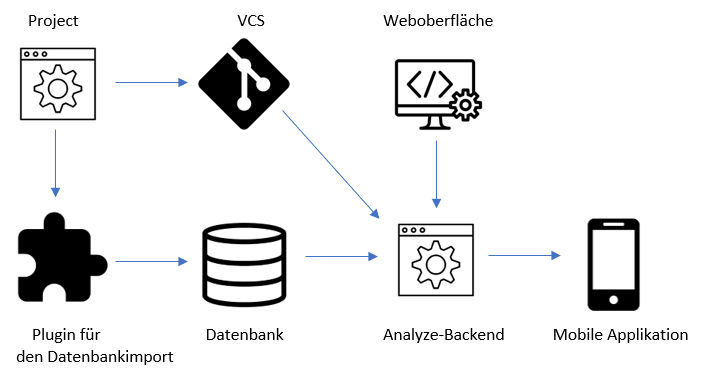
\includegraphics[height=8cm]{images/infrastruktur.PNG}
  % The short caption should be capitalised
  % The full caption should hold a full sentence. 
 \caption[Infrastruktur und beteiligte Applikationen und Systeme]{Infrastruktur sowie beteiligte Applikationen und Systeme. Die Pfeile zeigen hierbei den Datenfluss zwischen den einzelnen Systemen und Applikationen an.}
  \label{fig:findingsInIDE}
\end{figure}
\chapterend        % concept/design of solution
%%%%%%%%%%%%%%%%%%%%%%%%%%%%%%%%%%%%%%%%%%%%%%%%%%%%%%%%%%%%%%%%%%%%%%%%%%%%%
\chapter{Umsetzung}
\label{chap:Umsetzung}
%%%%%%%%%%%%%%%%%%%%%%%%%%%%%%%%%%%%%%%%%%%%%%%%%%%%%%%%%%%%%%%%%%%%%%%%%%%%%

\section{Technologien}
\subsection{Java}
Die drei Teilprojekte der Arbeit wurden in Java entwickelt. Die verwendete Java Version ist Java 11. Java wird als plattformunabhängige und robuste Programmiersprache verwendet. Auch in der Entwicklung der mobilen Applikation wird Java eingesetzt. Als Alternative zu Java könnte C-Sharp oder eine JavaScript basierende Webserver-Lösung wie Node.js fungieren.
\subsection{Android}
Die mobile Applikation ist eine Android-Anwendung. Als Programmiersprache wurde Java verwendet. Eine gute Alternative zu Java bietet Kotlin, da der Code kompakter und einfacher zu schreiben ist ~\parencite{banerjee2018comparative}. Aus Gründen der Einfachheit und Lesbarkeit wurde aber die Programmiersprache Java für die Entwicklung in Android gewählt. Ebenso bietet Android NDK (Native Development Kit) eine Alternative, mit der die mobile Applikation in C oder C++ entwickelt wird. Mit Android NDK kann schneller und wiederverwendbarer Code geschrieben werden, da der Code auch für andere Plattformen verwendet werden kann ~\parencite{ratabouil2015android}. Die Applikation wurde sowohl mit einem virtuellen Android-Emulator, als auch mit einem Android-Device getestet.
\subsection{Spring}
Spring, bzw. Spring Boot ist ein Java Framework, das im Zuge der Projektarbeit zur Entwicklungder Web-Applikation verwendet wurde. Spring Boot bietet zusätzlich unter anderem einen eingebetteten Server,  mit dem die Applikation schnell und einfach gestartet werden kann. Auch die Userverwaltung und damit auch die Security-Aspekte wurden mit Spring (Spring Security) entwickelt. Als mögliche Alternative zu Spring mit Spring Security kann Java EE mit einem OAuth2 eingesetzt werden. \ref{pressmarSpring}
\subsection{Maven und Gradle}
Maven ist ein Versionsverwaltungstool mit dem Abhängigkeiten und JARs verwaltetund heruntergeladen werden können. Maven wird hierbei in der Webapplikation und im Plugin eingesetzt. Eine Alternative zu Maven ist das Tool Gradle, welches in der Android Applikation für das Build-Management eingesetzt wurde.
\subsection{Thymeleaf}
Tyhmeleaf ist eine Template-Engine, die in HTML eingesetzt werden kann. Eine Template-Engine nimmt ein vorgefertigtes HTML-Skript (Template) und initialisiert dynamische Werte in die angegebenen Platzhalter. Thymeleaf gehört zu den Server-Side-Engines, das heißt die angezeigte Seite wird am Server generiert ~\parencite{searchmetrics}. Thymeleaf wird in der Webapplikation verwendet, um die Userverwaltung in der Weboberfläche zu implementieren. Der Vorteil dabei ist, da so eine einfache Interaktion mit dem Server stattfinden kann. Diese Interaktion ist beispielsweise die Anmeldung, bei der das angegebene Passwort validiert, überprüft und eine Validierungsnachricht zurückgegeben wird. Als Alternative kann JSF eingesetzt werden. 
\subsection{MongoDB}
Als Datenbank wird die nicht-relationale Lösung MongoDB verwendet, da es verschie-dene Vorteile gegenüber relationales Datenbankmanagementsystem bietet (siehe Punkt4.4.1). Es gehört zu den dokumentorientierten Datenbanken. MongoDB kann über die offiziele Website heruntergeladen und installiert werden. \footnote{https://www.mongodb.com/try/download/community}
\subsection{MongoDB Java Driver}
Der MongoDB Java Driver wird für die Kommunikation (Synchronisation und asyn-chrone Interaktion) mit MongoDB eingesetzt. Mit dem Driver werden unter anderem erstellten Benutzer in die Datenbank gespeichert und ausgelesen.
\subsection{IntelliJ und Android Studio}
Als Entwicklungsumgebungen wurden IntelliJ und Android Studio gewählt, da diese IDEs mehrere verschiedene Sprachen unterstützen und Android Studio eine Abwandlung von IntelliJ ist und daher die Entwicklung sehr einfach und nur minimal unterschiedlich ist.
\subsection{Git und SourceTree}
Git wurde für die Versionsverwaltung verwendet. Ebenso wird in der Applikation mit Git über eine GithubAPI kommuniziert und Daten abgefragt. \footnote{https://developer.github.com/v3/} (siehe Punkt 3.2.1 Konzept: Webapplikation). Statt Git kann auch die Software SVN(Apache Subversion) eingesetzt werden, welches aber verschiedene Nachteile hat wie ein schweres Branch-Handling. Als Git-basiertes Versionsverwaltung-Managementtool wird SourceTree verwendet.
\subsection{HTML, JavaScript und CSS}
Die Weboberfläche wurde mit diesen Technologien entwickelt. Ebenso wurden verschiedene JavaScript-Plugins und das CSS/JS-Framework Bootstrap verwendet, mit dem schnell und einfach Weboberfläche gestaltet werden können. Als Alternative zu HTML dienen Frameworks wie JavaEE Technologie JSF (Java Server Faces).
\section{Userverwaltung}
\subsection{Vorteile der Userverwaltung}
Ein Usermanagement mit Sicherheitsimplementierungen ist ein integraler und wichtiger Teil einer Webapplikation, in der sensible Daten behandelt werden, ebenso eignet sich in den gegebenen Anwendungsfällen eine Benutzerverwaltung besonders. Die Userwaltung ergibt daher folgende Vorteile:
\begin{itemize} 
  \item \textbf{Unterstützung für den Benutzer/die Benutzerin} 
Mit der Unterstützung der Userverwaltung können genauere Informationen und Berichte für den angemeldeten Benutzer angezeigt werden. Voraussetzung dafür ist aber die Integration und Verwendung eines Versionsverwaltungs-Management-Tools. So können die Fehler und Probleme der erstellten Files den Entwickler oder der Entwicklerin zugeordnet werden, welcher auf der Weboberfläche eingesehen werden können. So kann der User seine Fehler überblicken und gezielt ausbessern. Durch diese Individualisierung kann auch eine mögliche Verbesserung der Entwicklungsfähigkeit eintreten.  
    \item \textbf{Sicherheit und Zugriffsschutz} \\ Ein anderer wichtiger Punkt ist der Security-Aspekt. Die Webapplikation kann sowohl in einem Unternehmen, oder privat auf einem eigenen Server installiert werden. In beiden Fällen ist ein Zugriffsschutz notwendig, um unberechtigten Benutzer den Zugriff zu verweigern und sensible Daten zu schützen. Die Daten, die in der Webapplikation angezeigt werden müssen sehr vertraulich behandelt werden, da in der Weboberfläche neben weniger wichtigen Code-Smells auch zum Beispiel Sicherheitsprobleme angezeigt werden können. Diese Sicherheitsprobleme können von Angreifern ausgenutzt werden. Auch wenn die Applikation in einem gesicherten Firmennetzwerk installiert wird, ist die Implementierung eines Zugriffsschutzes wichtig. 
\item \textbf{Unterstützung für das Team}
Eigene Entwicklungsteams werden mithilfe einer Benutzerverwaltung erstellt. Dazu können zu den einzelnen Projekten Entwicklerinnen, Entwickler und andere am Projekt beteiligten Personen (Scrum-Master, Tester, usw.) hinzugefügt werden. Nur Mitglieder in diesen Teams können so die Fehler und Bugs einsehen. Den Usern werden daher nur die Projekte angezeigt, an welchen sie auch beteiligt sind. Außerdem können mithilfe der User- und Teamverwaltung eigene und spezielle Reports erstellt werden.
\end{itemize}

\subsection{Allgemeiner Aufbau} 
\subsubsection{User Flow}
Die Benutzerin oder der Benutzer sehen beim Aufrufen der Website, automatisch den Login. Ohne einer richtigen Anmeldung, kann man nicht auf die API oder die Webanwendung zugreifen. Der Benutzerin, der Benutzer muss sich vorher mit einer Email-Adresse und einem Passwort registrieren. Wenn eine Abmeldung nicht manuell erfolgt, so wird der User automatisch abgemeldet.
\subsubsection{Berechtigung zur Datenanzeige}
Um auf Projekt-Inhalte zugreifen zu können, muss ein Projektmitglied die Email-Adresse des neuen Teammitglieds zum Projekt hinzufügen. Erst wenn die Email-Adresse für das Projekt hinterlegt ist, werden die Fehler und Bugs des Projekts angezeigt. Eine andere Möglichkeit dieses Sicherheitsmechanismus wäre eine Anfrage der Entwicklerin oder des Entwicklers an das Team, welches dann die Email-Adresse akzeptieren oder ablehnen kann. So können keine unberechtigten Personen auf sensible Daten zugreifen. Eine Hierarchie-Regelung bzw. verschiedene Berechtigungsstufen sind nicht implementiert, da das Projektteam als Scrum-Team angesehen wird und im Scrum-Prozess alle Mitglieder gleichberechtigt sind \ref{scrumprozess}. Jedes Teammitglied kann daher ein neues Teammitglied mit der Email-Adresse hinzufügen.
\subsubsection{Administrator und initialer Zugriff}
Werden mit dem Datenbank-Importer-Plugin die Ergebnisse der Statischen Code Analyse eines bestimmten Projekts zum ersten Mal in die Datenbank geladen, so wird eine initiale Projektkonfiguration angelegt. Als erstes Mitglied wird automatisch ein Administrator gewählt. Dieser Administrator kann dann die ersten Teammitglieder, zum Beispiel die Projektleiterin oder den Projektleiter, in das Team einladen. So wurde das Problem gelöst, dass User zu Projekten nur eingeladen, aber nicht beitreten können. Ohne diese Implementierung kann aber kein User einen anderen User einladen, da zuerst kein User Mitglied des Teams ist. Die Mail-Adresse dieses Administrators muss im Plugin angegeben werden. Bei wiederholten Importen aus dem gleichen Projekt in die Datenbank, wird keine neue Konfiguration mehr erstellt.

\subsection{Implementierung des Usermanagements mit Spring Security}
\subsubsection{Allgemein}
Die Benutzerinnen und Benutzer werden in der Datenbank gespeichert. In der Datenbank wird dazu eine eigene Collection für die User angelegt. Die Passwörter werden verschlüsselt. In der Weboberfläche werden die Daten in einer Thymeleaf-UI eingegeben. Dazu müssen die Dependencies \textit{thymeleaf-layout-dialect} und \textit{spring-boot-starter-security} eingebunden werden. 
\subsubsection{Security Service}   
Im Security Service werden die Userdaten ausgelesen und gespeichert. Das Service implementiert die Spring-Security Schnittstelle \textit{UserDetailsService}. Beim Speichern wird das Passwort des an die Methode übergebenen Users überschrieben (siehe \ref{lst:phase}). Der \textit{BCryptPasswordEncoder} wird hierbei von Spring definiert und verschlüsselt das Passwort als Hash \footnote{https://docs.spring.io/spring-security/site/docs/4.2.15.RELEASE/apidocs/org/springframework/security/crypto/bcrypt/BCryptPasswordEncoder.html}. 

\lstset{
  caption={Speichern und Auslesen des Users. Beim Speichern des Benutzers wird das Passwort automatisch verschlüsselt.}, 
  basicstyle=\small\ttfamily, 
  label=lst:phase, 
  %float=tbhp, % float image to top/bottom/here/page
  language=Java,
  frame=single,
  breaklines=true, % break long source code lines, and add arrow
  postbreak=\mbox{\textcolor{red}{$\hookrightarrow$}\space},
  %  basewidth={0.55em}, 
  % fontadjust}  % adjust these for more appealing appearance
}

% listing with some settings, such as float, for this listing only
\begin{samepage}% with samepage we keep a FLOATing listing on one page
	\begin{lstlisting}[float=tbhp]
@Autowired
private BCryptPasswordEncoder passwordEncoder;

public void saveUser(User user) {
    user.setPassword(
       passwordEncoder.encode(user.getPassword()));
    mpngoUserService.saveUser(user);
}

@Override
public UserDetails loadUserByUsername(String email) 
  throws UsernameNotFoundException {

    User user = passwordEncoder.findByEmail(email);
    if (user != null) {
      List<GrantedAuthority> authorities =     
        getUserAuthority(user.getRoles());
          return authenticateUser(user, authorities);
    } else {
          throw new UsernameNotFoundException
             ("username not found");
    }
}
	\end{lstlisting}
\end{samepage}
Die Passwort-Überprüfung und der Aufruf der Methode \textit{loadUserByUsername} wird hierbei von Spring selbst implementiert.  Dazu muss das Datenbank-Objekt \textit{User} zum Spring-Objekt \textit{UserDetails} gemappt und eine eigene Configuration-Klassen implementiert werden (siehe Listing \ref{lst:config}). Im Security-Service sind ebenso Berechtigungsüberprüfungen implementiert. Dazu müssen Rollen erstellt und den Benutzer zugewiesen werden. Diese Rollen bzw. Berechtigungen werden mithilfe der \textit{GrantedAuthority} gespeichert und ausgelesen.

\lstset{
  caption={Konfiguration für das Spring Security UserService. Das Service \textit{UserSecurityService} wird nun als das zentrale Service für die Useroperationen von Spring Security verwendet.}, 
  basicstyle=\small\ttfamily, 
  label=lst:config, 
  %float=tbhp, % float image to top/bottom/here/page
  language=Java,
  frame=single,
  breaklines=true, % break long source code lines, and add arrow
  postbreak=\mbox{\textcolor{red}{$\hookrightarrow$}\space},
  %  basewidth={0.55em}, 
  % fontadjust}  % adjust these for more appealing appearance
}

% listing with some settings, such as float, for this listing only
\begin{samepage}% with samepage we keep a FLOATing listing on one page
	\begin{lstlisting}[float=tbhp]
@Bean
public UserDetailsService userDetailService() {
    return new UserSecurityService();
}

@Override
protected void configure
   (AuthenticationManagerBuilder auth) throws Exception {
     UserDetailsService detailsService = userDetailService();
     auth.userDetailsService(detailsService)
        .passwordEncoder(bCryptPasswordEncoder);
}
	\end{lstlisting}
\end{samepage}
Werden hier andere Datenbanken oder Services implementiert, so muss nur die Implementation für das Repository bzw. in diesem Fall das \textit{mpngoUserService} ausgetauscht werden. 
\subsubsection{Security Konfigurationen}
Um die Applikation (URLs der einzelnen Unterseiten) und die API schützen zu können, müssen nun weitere Konfigurationen hinzugefügt werden ~\parencite{springSecBook}. Dazu müssen die einzelnen URLs für die Anzeige der Daten gesichert werden, während hingegen die URLs für den Login und den Website-Aufruf frei zugänglich sein müssen. Auch die Logout-URL kann hier angegeben werden \ref{lst:configurls}.
\lstset{
  caption=[Konfiguration für die Sicherheit der URLs.]{Konfiguration für die Sicherheit der URLs. Die einzelnen Paths können entweder für alle freigegeben oder für eine bestimmte Gruppe angezeigt werden. Das Abmelden wird von Spring automatisch durchgeführt.}, 
  basicstyle=\small\ttfamily, 
  label=lst:configurls, 
  %float=tbhp, % float image to top/bottom/here/page
  language=Java,
  frame=single,
  breaklines=true, % break long source code lines, and add arrow
  postbreak=\mbox{\textcolor{red}{$\hookrightarrow$}\space},
  %  basewidth={0.55em}, 
  % fontadjust}  % adjust these for more appealing appearance
}

% listing with some settings, such as float, for this listing only
\begin{samepage}% with samepage we keep a FLOATing listing on one page
	\begin{lstlisting}[float=tbhp]
...
http.antMatchers("/login").permitAll()
.antMatchers("/reports").hasAuthority("USER")
.and().logout()
.logoutRequestMatcher(new AntPathRequestMatcher("/logout"))
\end{lstlisting}
\end{samepage}
Um auf den Login reagieren zu können, wird ein \textit{AuthenticationSuccessHandler} verwendet, der nach dem Login den User auf die Weboberfläche der Datenanzeige weiterleitet. Hierbei sind im \textit{AuthenticationSuccessHandler} auch noch Überprüfungen implementiert, die den User je nach Rolle (Admin oder User) weiterleiten. 
\subsubsection{Controller und Oberfläche} 
Im Gegensatz zu den anderen Teilen der Webapplikation ist der Login mit Thymeleaf erstellt worden, da so die Login-Überprüfung und das Handling einfach implementiert werden kann. Auch die Navigationsleiste ist mit Thymeleaf implementiert, um auch die Logout-Funktion einfach zu gestalten. Ebenso kann in der Navigationsleiste der angemeldete User eingesehen werden (siehe Abbildung \ref{fig:configuration}). Um Thymeleaf verwenden zu können, ist ein Controller implementiert, der zu den Thymeleaf-Seiten Get-Methoden mit einer \textit{ModelAndView} zur Verfügung stellt. Im \textit{ModelAndView} wird das Model (User) und die View (z.B. Thymeleaf-Login-Page) gespeichert. Als Get-Path wird der Pfad des Thymeleaf-Templates angegeben ~\parencite[Seite 160]{springSecBook}. In der Weboberfläche kann so einfach auf die Daten des Users, zum Beispiel Name und Rechte, zugegriffen werden.
\subsection{Projektkonfiguration für Teammitglieder}
In der Unterseite \textit{Configuration} können die Teammitglieder des Projekts angezeigt und neue Teammitglieder hinzugefügt werden. Dazu muss der angemeldete Benutzer selbst Teil des Teams sein. Um eine neuen User zum Projekt hinzuzufügen muss die Email angegeben werden (siehe Abbildung \ref{fig:configuration}). Der eingeladene User kann daraufhin die Daten des Projekts (Fehler, Bugs, Errors, Charts, usw.) auf der Webseite einsehen. Auf der Konfigurationsseite kann auch eine Projektbeschreibung und ein Link für die Versionsverwaltung hinzugefügt werden (siehe Punkt TODO). Dieser Link dient zur persönlichen Fehler- und Meldungsanzeige sowie zur Verlinkung zum Einsehen der Fehler. (siehe Punkt TODO). Die Konfigurationen für jedes Projekt werden in einer eigenen MongoDB-Collection \textit{configurations} gespeichert. Dieser Eintrag wird initial ohne Konfigurationen beim ersten Import mit dem Importer-Plugin  erstellt.
\begin{figure}[tp]
  \centering
  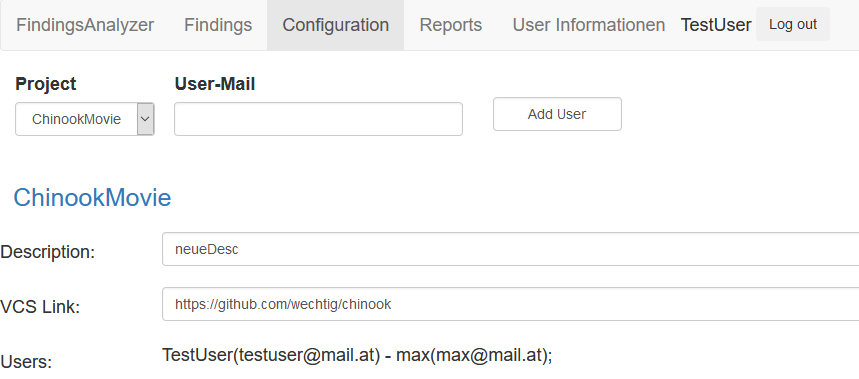
\includegraphics[height=6cm]{images/configuration.PNG}
  % The short caption should be capitalised
  % The full caption should hold a full sentence. 
 \caption[Konfiguration für das Projekt und Team]{Unterseite für verschiedene Konfigurationen für das Projekt und das Team. In diesem Beispiel ist der angemeldete User \textit{TestUser} Mitglied des Teams für das Projekt \textit{ChinookMovie}. So kann er neue Mitglieder zum Team hinzufügen.}
  \label{fig:configuration}
\end{figure}
\section{Anbindung der Versionsverwaltung für spezifische User-Unterstützung}
\subsection{Allgemeines}
Auf der Hauptseite der Webapplikation werden alle Fehler, Code Smells, Warnungen und Bugs gelistet, die die Tools der Statischen Code Analyse im Projekt finden und welche mit den Importer-Plugin in die Datenbank importiert werden. Diese Informationen werden alle in einer Tabelle angezeigt, welche nach Projekt, Klasse oder Datum sortiert und gefiltert werden kann. \\
Das Problem bei dieser Implementierung ist die unspezifische Anzeige: Den Teammitgliedern werden alle Informationen angezeigt, auch Fehler, die von anderen Entwicklerinnen oder Entwicklern implementiert worden sind. So können  Fehler im Projekt gefunden werden und das Team kann die Fehler einsehen. Das Problem bei einer dauerhaften Verbesserung der Kenntnisse der Entwicklerinnen und Entwickler ist hierbei aber die unpersönliche Anzeige. Um den Usern der Webapplikation die genauen Fehler anzuzeigen wird Lösung mit der Anbindung eines VCS-Tools (Version Control System) implementiert. Das Konzept dabei ist es, das die angemeldeten User mit den VCS-Usern verbunden werden. So können die genauen Implementierungen untersucht werden. Dabei werden zum Beispiel die committeden Klassen aus den einzelnen gelesen.
\subsubsection{Ablauf}
Um die spezifische User Unterstützung benutzen zu können, muss im Projekt eine Versionsverwaltung verwendet werden (Im Rahmen dieser Arbeit wurde hierbei die Unterstützung für die Versionsverwaltung Git implementiert). Der Link des Repositories muss zusätzlich in der Projektkonfiguration von einem Teammitglied konfiguriert werden (siehe Abbildung 4.1). Um nun die Accounts der Teammitglieder in der Userverwaltung mit den Entwicklerinnen und Entwicklern des Projekts in der Versionsverwaltung verbinden zu können, wird die Email-Adresse verwendet. Das heißt, die Email-Adresse im Tool der Versionsverwaltung muss mit der Email-Adresse der Userverwaltung übereinstimmen. Werden nun in der Weboberfläche die Informationen zu der Statischen Code Analyse abgefragt, so werden die Informationen in der Datenbank mit den Daten der Versionsverwaltungs-API verglichen und es wird versucht eine Verbindung herzustellen. Es werden nur jene Fehler und Informationen abgefragt und angezeigt, die vom angemeldeten User implementiert und committed worden sind.   
\subsubsection{Alternative Implementierungsmöglichkeiten}
Die beschriebene Methode mit der Einbeziehung eines Versionsverwaltungstools ist nur eine mögliche Methode zur persönlichen Anzeige. Ein Problem bei dieser Methode ist die verpflichtende Angabe eines VCS-Links. Andere Möglichkeiten, die diese Konfiguration nicht verlangen, sind unter anderem: \\
\textbf{Angabe der entwickelnden Klassen und Methoden} \\
Hierbei könnten die Entwicklerinnen und Entwickler die entwickelnden Methoden und Klassen in einer Übersichtsseite auswählen. Fehler, Bugs und andere Meldungen aus diesen Klassen werden den Usern angezeigt.\\
\textbf{Automatische Erkennung durch Verteilung der Aufgaben} \\
Die Idee bei dieser Methode ist eine Konfiguration, wo die Aufgaben verteilt werden: Die Benutzerinnen und Benutzer könnten hierbei jene Packages oder Module angeben, welche sie entwickeln. So können zum Beispiel die Aufgaben als Packages wie Repositories, Modules oder Weboberfläche verteilt werden. \\
\textbf{Autorennamen verwenden} \\
Bei dieser möglichen Lösung werden die Autorangaben der \textit{Javadoc} verwendet. Bei der \textit{Javadoc} zu Klassen werden unter anderem die Autoren angegeben \footnote{https://www.oracle.com/technical-resources/articles/java/javadoc-tool.html}. Dieser Autorenname kann dazu verwendet werden, um den angemeldeten Usern die richtigen Meldungen anzuzeigen, wenn die beiden Namen übereinstimmen.
\subsection{GithubAPI und Service}
Mit der GithubAPI können anderem die Commits eines Repositories abgefragt werden. Dazu müssen der User und der Name des Repositories bekannt sein. Um genauere Abfragen zu erstellen, wird auch ein Datumsbereich angegeben. Aus diesen Variablen wird ein Pfad erstellt, mit dem die Daten abgefragt werden (siehe 4.3.2.1). Der Pfad zum Repository muss in der Oberfläche für die Konfiguration angeben werden, die anderen Daten kann die Benutzerin oder der Benutzer bei der Abfrage auf der Weboberfläche auswählen. 
\subsubsection{HttpClient und API-Abfrage}
Der \textit{HttpClient} ist seit Java 11 ein Teil von Java \footnote{https://openjdk.java.net/groups/net/httpclient/intro.html}. Mit dem HttpClient können unter anderem Http-Daten abgefragt werden. Der \textit{HttpClient} wird in der Arbeit dazu verwendet, um die Daten der GithubAPI abzufragen. Dazu wird der Github-API-Pfad verwendet. Der \textit{HttpClient} benötigt zur Abfrage noch einen \textit{HttpRequest} um den Request abzuschicken und zu verarbeiten. Im \textit{HttpRequest} können Header-Variablen(User-Agent) und die Http-Methode(Bei der Github-Abfrage die Methode \textit{GET}) angegeben werden. Der Rückgabewert kann mit dem \textit{HttpResponse} bearbeitet werden (siehe Listing   \ref{lst:httprequest}).
\lstset{
  caption=[Listing für die Implementierung für die Abfrage der Github-API und Beispiel-Request.]{Listing für die Implementierung für die Abfrage der Github-API. Am Beginn des Listings wird in einem Kommentar ein Beispiel-Link für den Request angezeigt. Im Link enthalten ist der Benutzername des Users und der Datumsbereich, aus dem die Commits geladen werden sollen.}, 
  basicstyle=\small\ttfamily, 
  label=lst:httprequest, 
  %float=tbhp, % float image to top/bottom/here/page
  language=Java,
  frame=single,
  breaklines=true, % break long source code lines, and add arrow
  postbreak=\mbox{\textcolor{red}{$\hookrightarrow$}\space},
  %  basewidth={0.55em}, 
  % fontadjust}  % adjust these for more appealing appearance
}
\begin{samepage}% with samepage we keep a FLOATing listing on one page
	\begin{lstlisting}[float=tbhp]
https://api.github.com/repos/wechtig
/chinook/commits?since=2014-07-29&until=2020-07-28
...
HttpClient httpClient = HttpClient.newBuilder()
     .version(HttpClient.Version.HTTP_1_1)
     .connectTimeout(Duration.ofSeconds(20))
     .build();

public String get(String url)  {
    HttpRequest request = HttpRequest.newBuilder()
     .GET()
     .uri(URI.create(url))
     .setHeader("User-Agent", "Java 11 HttpClient Bot")
     .build();
    try {
      HttpResponse<String> response = 
      httpClient.send
      	(request, HttpResponse.BodyHandlers.ofString());
            return response.body();
	...
	\end{lstlisting}
\end{samepage}
\subsubsection{Verarbeitung des Response}
Der \textit{HttpResponse} beinhaltet neben Informationen wie den Http-Status-Code, verschiedenen Headers und anderen Variablen einen Response-Body. Dieser Body kann als JSON gelesen und verwendet werden. Die JSON-Werte werden mit Java als \textit{Map} mit zwei \textit{String} gelesen. So kann der Variablenname und der Wert gelesen werden. Da sich im Response mehrere JSON-Werte befinden, muss zusätzlich eine Liste erstellt werden. Aus dem Response können nun die Autoren und die Commit-Links ausgelesen werden. Es werden nur jene Commits in der Liste gespeichert, wo der Autor mit dem angemeldeten Benutzer übereinstimmt. Commits von anderen Entwicklerinnen oder Entwickler werden nicht gespeichert, da sie nicht in der persönlichen Fehler- und Buganzeige auftauchen sollen. Die einzelnen Änderungen können nur über die Commit-Links herausgefunden werden, daher muss ein zweiter Request abgeschickt werden. Aus dem Response des zweiten Commit-Requests lassen sich nun die geänderten Datein (filename) auslesen \ref{lst:lstresponse}. Dazu kann der \textit{ObjectMapper} verwendet werden.
\lstset{
  caption=[Auslesen der geänderten Files aus der Github-API.]{Auslesen der geänderten Files aus der Github-API. Die Links für die Commits müssen in einem eigenen Request vom Repository ausgelesen werden.}, 
  basicstyle=\small\ttfamily, 
  label=lst:lstresponse, 
  %float=tbhp, % float image to top/bottom/here/page
  language=Java,
  frame=single,
  breaklines=true, % break long source code lines, and add arrow
  postbreak=\mbox{\textcolor{red}{$\hookrightarrow$}\space},
  %  basewidth={0.55em}, 
  % fontadjust}  % adjust these for more appealing appearance
}
\begin{samepage}% with samepage we keep a FLOATing listing on one page
	\begin{lstlisting}[float=tbhp]
...
List<String> files = new ArrayList<>();
for (String commit : commitLinks) {
   String commitData = httpGithubClient.get(commit);
   if(data == null) {
       return new ArrayList<>();
   }
   try {
     Map<String, List<Object>> commitResponse = new   
      ObjectMapper().readValue(commitData, Map.class);
     List<Object> changedFiles = 
      commitResponse.get("files");

     if(changedFiles == null) {
      continue;
     }

     for(Object o : changedFiles)  {
      String filename = 
        (String) ((LinkedHashMap) o).get("filename");
      files.add(filename);
     }
...     
	\end{lstlisting}
\end{samepage}
Nachdem die geänderten Dateien ausgelesen worden sind, werden aus der Datenbank die Fehlerinformationen und Warnung für die Datei gelesen. Bei der Datenabfrage wird auch der Datumsbereich verwendet, um genauere Anzeigen zu bekommen.
\subsection{Fehlende Informationen über die geänderten Zeilen}
Ein Problem bei der Unterstützung der GithubAPI, ist die fehlende Information über die genauen geänderten Zeilen. Denn mit der GithubAPI ist es nur möglich, die geänderten Dateien auszulesen, nicht aber genaue die geänderten Zeilen. So ist es möglich, das ein anderes Teammitglied den Fehler bereits früher in die Klasse eingebaut hat. Wenn die Klasse beim Commit geändert wird, so wird auch dieser Fehler angezeigt. Wenn aber eine Entwicklerin oder ein Entwickler Änderungen an einer Klasse vorgenommen hat und Fehler übersehen oder nicht die Kenntnisse über den Fehler hat, so ist es auch ein möglicher Vorteil für das Teammitglied, wenn der Fehler in der Übersicht angezeigt wird. 
\subsection{Oberfläche}
Die Oberfläche für die persönliche Fehler und Warnungsanzeige des Users ist identisch mit der allgemeinen Übersichtsansicht. Zusätzlich wurde aber eine Github-Verlinkung für die Fehler in der Tabelle eingebaut. Dieser Link wurde auf die Anzeige der betreffenden Zeilennummer gesetzt (TODO siehe Abbildung Kommentare). Über diesen Link kann der Code in der Online-Versionsverwaltung eingesehen werden. Der Link wird hierbei aus dem Link für das Repository in der Konfiguration, aus dem Filenamen und den Zeilennummern erstellt. Dadurch, dass im Link die Zeilennummern hinzugefügt werden, kann die genaue Zeile angezeigt werden. Auch Fehler, die sich über mehrere Zeilen strecken, werden markiert (siehe Abbildung \ref{fig:markedFindings}). 
\begin{figure}[tp]
  \centering
  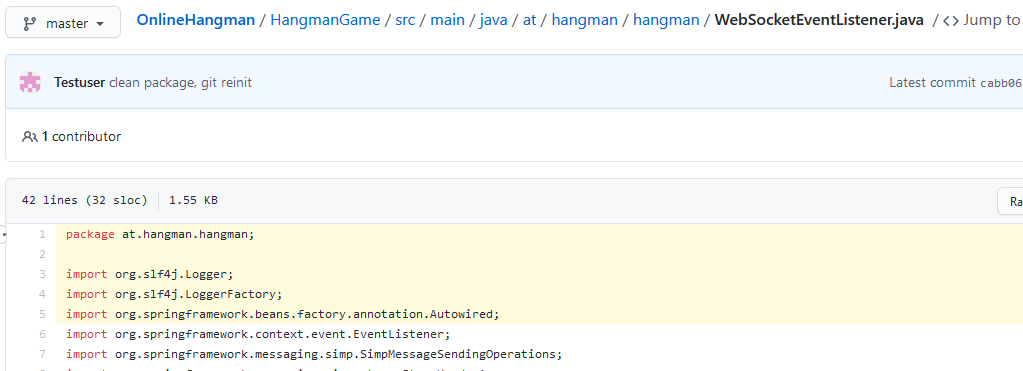
\includegraphics[height=5cm]{images/markedFindings.PNG}
  % The short caption should be capitalised
  % The full caption should hold a full sentence. 
 \caption[Anzeige der markierten Fehler]{Über einen Link kann der Fehler im Code genau markiert und angezeigt werden.}
  \label{fig:markedFindings}
\end{figure}
\section{Cron Job und Report Sender für Berichte}
\subsection{Automatische Berichte} 
Mit dem Cron Job Reporter können Teams regelmäßige Berichte vom Projekt direkt erhalten. Die Reports von einem Projekt werden direkt an alle Teammitglieder geschickt. So können die wichtigsten Informationen, Charts und Änderungen eingesehen werden, ohne dass die Webapplikation benutzt werden muss. Dieser Bericht soll regelmäßig (Einmal in der Woche) automatisch versendet werden. Dafür wird ein Cron Job verwendet. Der automatische Bericht kann unter anderen für Projektmanager oder Scrum-Master verwendet werden, welche an mehreren verschiedene Projekten beteiligt sind. Aber auch die Entwicklerinnen und Entwickler können so schnell die neuesten Änderungen einsehen. \\ Ein Cron Job bzw. ein Scheduler ist eine Implementierung, die einen bestimmten Task immer wieder zu einem bestimmten Zeitpunkt ausführt. Spring bietet die Möglichkeit, solche Scheduler zu erstellen. Dazu muss das Keyword \textit{Scheduled} zusammen mit einer Cron-Expression verwendet werden ~\parencite{cintirScheduler}. Diese Konfiguration wird bei einer Methode angewandt, welche die neuen Fehler und Warnungen der letzten Woche aus der Datenbank ausliest und daraus einen Report generiert. Ebenso werden die Charts eingebunden. Der Report wird danach mit dem Mail-Cient versendet (siehe 4.4.3). Mit einer Cron-Expression kann der Zeitpunkt festgelegt werden, wann die Berichte versendet werden sollen. Die Cron-Expression kann im File \textit{application.yml}(YAML-Framework) definiert werden, der Standardwert der Cron-Expression ist \textit{0 0 12 ? * 6}, also jeden Freitag um 12:00. Das YAML-Framwork ist ein Framework für die einfache Serealisierung von Daten, also für die Persistierung eines Objekts um Daten und Informationen zu speichern ~\parencite{eriksson2011comparison}. So können die Informationen einfach gespeichert und ausgelesen werden. In Spring kann aber zur Alternative das File \textit{application.properties} verwendet werden. \\ Um den Scheduler bei der Spring-Security verwenden zu können, muss bei den Sicherheitskonfiguration (\textit{WebSecurityConfigurerAdapter}) der Scheduler zugelassen werden. Für den Spring Scheduler können eigene XML-Konfigurationsdateien erstellt werden, in der zum Beispiel die Cron-Expression auch definiert werden kann.
\subsection{Manuelle Berichte}
Auch manuell können Berichte an bestimmte Personen verschickt werden. Für das manuelle Versenden der Berichte gibt es in der Webapplikation eine eigenen Unterseite: \textit{Reports}. Dort kann das Projekt und der Zeitraum ausgewählt werden, aus welchen der Report generiert werden soll. Der generierte Report kann an das Team oder an eine selbst gewählte Email-Adresse versendet werden. Ebenso kann auch ausgewählt werden, ob der Bericht nur die Charts beinhalten soll oder auch ein Listing der neuen Fehler und Meldungen.
\subsection{Versenden der Reports mit Java Mail}
Der PDF-Report wird aus den Daten mit iText-PDF generiert (siehe Bacherlorarbeit 1). Die Charts werden ebenso in den PDF-Report eingefügt. Erstellt werden die Charts aber mit dem JavaScript-Framework Chart.js im Frontend und sie werden nach der Generierung an den Server übermittelt. Die Charts werden am Server mit dem Informationen wie Zeitraum der Daten und Projektname gespeichert. So können die Charts bei der Generierung vom Server geladen und eingefügt werden. Die PDF-Reports werden nach der Erstellung mit dem Java-Mail Client versendet. 
\subsubsection{Implementierung und Konfiguration} 
Aus den Daten und Reports wird mit JavaMail eine \textit{MimeMessage} generiert. Bei einer \textit{MimeMessage} können Informationen wie Empfänger, Anhang, Text und Betreff angegeben werden ~\parencite{harold2013javamail}. Da eine PDF an die Mail angehängt wird, muss auch ein \textit{MimePart} angegeben werden, indem der Datentyp PDF definert wird. Um eine \textit{MimeMessage} aber erstellen zu können, wird eine Session benötigt. Die Session kann ein Mail-Server sein, über diese Session wird also die Nachricht übermittelt. Da für die Arbeit kein eigener Mail-Server zur Verfügung stand, wurde ein einfacher Mail-Account angegeben. Die Mails werden dann über diesen Mail-Account gesendet. Für den Mail-Account muss eine Email-Adresse und das Passwort angegeben werden. Viele Mail-Programme blockieren aber initial eine solche Versendung der Mails, dies kann aber aktiviert werden. Nachdem die Session erstellt wurde, müssen noch Einstellung wie SMTP-Host, Port und andere Informationen angegeben werden. SMTP ist das Protokoll das verwendet werden muss, um die Emails versenden zu können. Als SMTP-Host wurde also bei der Arbeit der Gmail-Host verwendet (smtp.gmail.com). Der Gmail-Host kann aber nur verwendet werden, wenn gewisse Security-Einstellungen am Email-Account vorgenommen werden.Beim Einsatz der Applikation, beispielsweise in einem Unternehmen, kann der SMTP-Server durch einen eigenen internen SMTP-Server ersetzt werden.
\section{Kommentare}
\subsection{Allgemeines und Vergleich zu Pull Requests}
\begin{figure}[tp]
  \centering
  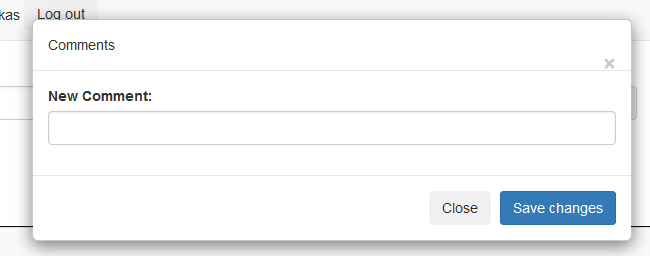
\includegraphics[height=5cm]{images/popup.PNG}
  % The short caption should be capitalised
  % The full caption should hold a full sentence. 
 \caption[Popup für das Speichern von Kommentaren]{Popup für das Speichern von Kommentaren. Beim Popup für das Anzeigen von Kommentaren wird das Eingabefeld durch ein Listing der Kommentare ersetzt.}
  \label{fig:table}
\end{figure}
Ein wichtiger Teil des Git-Workflows um Code Qualität sicher zustellen, sind die sogenannten \textit{Pull Requests} (siehe Kapitel 2.3). Pull Requests werden dazu verwendet, um neuen Code von einem bestimmten Branch (Zweig) in die gemeinsame Codebasis zu integrieren. Die Integration von fehlerhaften Code oder von Code mit schlechter Qualität soll vermieden werden. Bei Pull Requests werden daher Kommentare und Anmerkungen von anderen Teammitgliedern zu neuen Code erstellt. Werden Fehler oder Probleme bei Pull Request vom Reviewer festgestellt, bessert diese die Entwicklerin oder der Entwickler aus. \\ Mit der Kommentarfunktion können in der Weboberfläche die verschiedenen Meldungen von allen Teammitgliedern in der Übersichtstabelle kommentiert und angezeigt werden (siehe Abbildung \ref{fig:table}). Diese Kommentare unterscheiden sich von den Kommentaren in Pull Requests daher, dass sie Informationen für alle Entwicklerinnen und Entwickler darstellen. So können Kommentare, die Verbesserungsvorschläge oder andere hilfreiche Informationen beinhalten, den ganzen Team helfen. Ebenso werden diese Kommentare dauerhaft gespeichert und angezeigt werden, während Pull Requests gelöscht werden. Die Kommentare beziehen sich auch inhaltlich auf den Fehler und sollen Verbesserungsvorschläge beinhalten, während Kommentare in Pull Requests meist nur auf Fehler hinweisen. Bei der persönlichen Fehleranzeige können daher auch keine Kommentare hinzugefügt und angezeigt werden.
\subsection{Implementierung}
Um ein Kommentar speichern zu können, muss in der Übersichtstabelle das Kommentar-Popup geöffnet werden. In diesem Bootstrap-Popup kann das Kommentar eingegeben und gespeichert werden. Die Kommentare werden in einer eigenen Collection \textit{comments} gespeichert. Über einen eigenen Button können die Kommentare angezeigt werden (siehe Abbildung \ref{fig:popup}). Die Kommentare werden hierbei in das Popup geladen. \\ Wird der Datenbankimport wiederholt ausgeführ, um Informationen über einen längeren Zeitraum zu erhalten, so wird der selbe Fehler öfters in der Datenbank gespeichert.
\begin{figure}[tp]
  \centering
  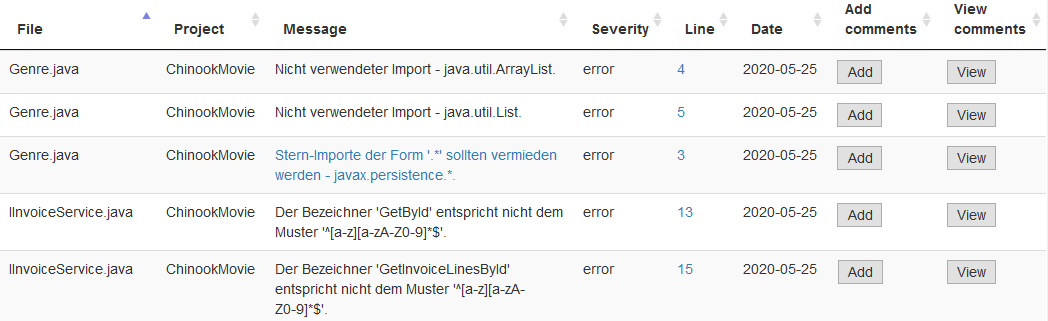
\includegraphics[height=5cm]{images/table.PNG}
  % The short caption should be capitalised
  % The full caption should hold a full sentence. 
 \caption[Übersichtstabelle]{Übersichtstabelle mit der Auflistung der Meldungen. Mit den zwei Buttons können die Kommentare erstellt und angezeigt werden. Die Zeilennummer ist ein Link für die Öffnung und Anzeige des Fehlers und des Codes in der Versionsverwaltung Github. Der Link kann nur erstellt werden, wenn in der Konfiguration das Repository angegeben ist. Die Tabelle wurde mit Pagination erstellt: So kann in der Tabelle navigiert werden, sodass nie die ganze Tabelle angezeigt wird. }
  \label{fig:popup}
\end{figure}
Ein Kommentar, das daher zu einer bestimmten Meldung erfasst wird, soll aber auch für die selben anderen Meldungen gelten, welche bei wiederholten Importen gespeichert werden. Daher wird beim Auslesen der Kommentare aus der Datenbank nicht eine bestimmte Identifikationsnummer benutzt, sondern die Attribute die das Kommentar bestimmen (Projekt, Klasse, Meldung, Zeile). So wird bei allen gleichen Meldungen der Kommentar angezeigt.
\section{Mobile Android Applikation}
\subsection{Allgemeines und Idee}
Die Android Applikation soll eine neue Möglichkeit sein, um die Code Qualität zu steigern. Die wichtigsten Informationen aus der Webapplikation sollen hierbei kompakt angezeigt werden: Die einzelnen Meldungen und die verschiedenen Charts. Die Möglichkeit zur Filterung nach Projekt und Zeitbereich soll auch hierbei verfügbar sein. Die Applikation wurde mit Java entwickelt. \\ Die Applikation verwendet keinen direkten Zugriff auf die Datenbank. So konnte unter anderem doppelter Code vermieden werden, da Services und Repositorys nicht für beiden Applikationen entwickelt werden . Die mobile Applikation bezieht die Daten aus der API der Webapplikation. Dazu werden mit verschieden Attributen HTTP-Requests abgeschickt. Die HTTP-Parameter die benötigt werden um die Daten aus der Datenbank abzufragen, kann die Benutzerin oder Benutzer beim Start der Applikation auswählen. Die Webapplikation wiederum liest die Daten mithilfe der Services und des MongoDB Java Drivers aus der Datenbank aus. Der Aufbau der Applikation beinhaltet Java-Packages für die Datenhaltungsklassen und die Business-Logik wie HTTP-Tasks, sowie auch die Aktivitäten (siehe Abbildung 4.5).

\begin{figure}[tp]
  \centering
  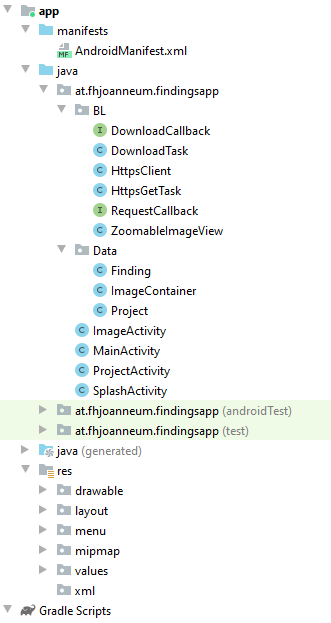
\includegraphics[height=8cm]{images/androidPackages.PNG}
  % The short caption should be capitalised
  % The full caption should hold a full sentence. 
 \caption[Aufbau und package-Struktur der Webapplikation]{Aufbau und package-Struktur der Webapplikation. Im package \textit{manifests} wird das Android-Manifest definiert. Die Datenhaltungsklassen, Aktivitäten und die Business-Logic befinden sich im Package \textit{java}. Im Folder \textit{res} befinden sich die Inhalte zum Layout der Applikation.}
  \label{fig:popup}
\end{figure}


\subsubsection{Neuer Funktion zur Steigerung der Kenntnisse}
In der Applikation soll ebenso ein neuer Aspekt oder eine neue Funktion implementiert werden, die der Unterstützung der Kenntnisse über bestimmte Fehler dient. Implementiert wurde so eine kleine spielerische Funktion, mit der die Entwicklerinnen und Entwickler unterstützt werden sollen. Diese Funktion wurde als Shake-Funktion entwickelt, mit der zufällige Inhalte angezeigt werden. Wird also das mobile Gerät geschüttelt, so werden zufällige Meldungen oder Charts angezeigt.
\subsection{Abfrage der Daten}
Um die Informationen verwendet zu können, wird ein Request verwendet. Der Request wird als HTTP-Get-Funktion implementiert. Mit den Informationen zu Projekt und Datumsbereich wird die URL erstellt. Mit einer \textit{HttpURLConnection} wird der Request abgeschickt ~\parencite{liu2017web}. Auch andere Http-Funktionen werden von der Klasse \textit{HttpURLConnection} unterstützt, daher muss die HTTP-Methode \textit{Get} aber auch andere Optionen wie das \textit{Timeout} angegeben werden. Der Request wird daraufhin vom Controller in der Webapplikation verarbeitet und eine Response enthält die Charts und Informationen. Ist der Response-Code der Wert 200 (OK), so wird der Response mit einem \textit{BufferedReader} und einem \textit{InputSream} gelesen. Die Daten werden an die Aktivität als JSON-Wert zurückgegeben. Um die Daten aus dem JSON-Result verwenden zu können wurde noch ein \textit{JSONArray} benutzt, von dem die verschiedenen \textit{JSONObjects} ausgelesen und zu Java-Objekten umgewandelt wurden. 
\subsection{Aktivitäten und Navigation}
Eine \textit{Activity} wird für einen bestimmte Anzeige, also zum Beispiel ein Formular oder ein Bildschirm, erstellt ~\parencite{mednieks2012programming}. Diese Aktivitäten werden im Android Manifest registriert. Ebenso kann zu den Aktivitäten eine Layout-Klasse erstellt werden. Diese Layout-Klasse wird in der \textit{Activity} registriert. Zwischen den einzelnen Aktivitäten soll der Benutzer wechseln können, entweder manuell oder automatisch. In der Applikation gibt es vier Aktivitäten (siehe Abbildung 4.6):
\subsubsection{SplashActivity}
Die SplashActivity wird zuerst initial ausgeführt. Dies kann im Android-Manifest mit der Option \textit{android.intent.category.LAUNCHER} festgelegt werden. Während des Startvorgangs wird ein \textit{SplashScreen} kurz angezeigt. Der Benutzer wird danach automatisch zur nächsten Aktivität weitergeleitet. Dieser Startbildschirm dient zur Information und zum Erstellen der Applikation und andere Ladevorgänge. \\ Während des \textit{SplashScreen} wird der erste Request erstellt: Hierbei werden von der Webapplikation die Projektdaten geladen. Mittels eines Intents wird die nächste Aktivität \textit{ProjectActivity} danach automatisch gestartet und die Projektdaten werden weitergegeben. Ein Intent ist eine klare Funktion oder Aufgabe in der Android-Applikation, zum Beispiel der Start einer anderen Aktivität ~\parencite{vogelIntent}.
\subsubsection{ProjectActivity}
In der \textit{ProjectActivity} werden die Projektdaten aus dem Intent ausgelesen. Die Projektnamen werden im dazugehörigen Layout in einer \textit{SelectBox} angezeigt. Ebenso gibt es im Projekt-Layout zwei Date-Picker, mit dem der Datumsbereich der Abfrage festgelegt werden kann. Nachdem die Benutzerin oder der Benutzer einen Datumsbereich und ein Projekt ausgewählt hat, wird die eingegebenen Daten in der Aktivität gespeichert. Nachdem die Benutzerin oder der Benutzer alle Daten eingegeben hat, wird automatisch die nächste Aktivität aufgerufen. Die ausgewählten Parameter Projektname und Datumsbereich werden wieder in einem Intent gespeichert und die nächste Aktivität wird automatisch aufgerufen.
\subsubsection{MainActivity}
Die \textit{MainActivity} ist die zentrale Aktivität der Applikation. Im Layout zur \textit{MainActivity} werden die Meldungen, Bugs und Fehler angezeigt. \\ Bevor die Aktivität angezeigt wird, werden die Parameter aus dem Intent gelesen. Mit diesen Parametern wird ein Request durchgeführt und die Meldungen werden im Backend der Webapplikation aus der Datenbank ausgelesen und zurückgegeben. Der Response wird in der mobilen Applikation zu einer Liste von Meldungen konvertiert. Aufgrund der Größe des Textes der Fehlermeldungen werden die Informationen nicht in einer gemeinsamen Liste oder auf einen Bildschirm angezeigt, sondern einzeln. Durch zwei Buttons im Footer kann die Benutzerin oder der Benutzer  nach vor oder zurück in der Liste navigieren und die Fehler genau einsehen. Dabei wird auch die Klasse und die Zeilennummer der Meldung angezeigt. Wird das mobile Geräte bei dieser Aktivität geschüttelt, so wird eine zufällige Meldung angezeigt (siehe Punkt 4.6.4). Ebenso gibt es im Footer ein Image-Icon, das die Möglichkeit bereitstellt, die generierten Charts, erstellt aus den Meldungen, anzuzeigen (siehe Bac 2 TODO). Wird diese Option ausgewählt, wird die Aktivität gewechselt, und die \textit{ImageActivity} aufgerufen.
\subsubsection{ImageActivity}
In der \textit{ImageActivity} werden die Parameter zunächst wieder ausgelesen. Mit den Parametern wird ein Request geschickt und die Charts von der Webapplikation geladen. Die Bilder werden in einer \textit{ImageView} im Layout angezeigt. Auch hierbei besteht wieder die Möglichkeit zwischen den Bildern zu navigieren. Ebenso wird auch ein zufälliges Charts angezeigt, wenn das mobile Gerät geschüttelt wird. Im Footer des Layouts zur \textit{ImageActivity} gibt es wieder die Option, zur \textit{MainActivity} zu wechseln. \\
\textbf{Fehlende Generierung der Charts am Backend} \\
Ein Problem bei dieser Lösung ist, das die Charts nicht im Backend der Webapplikation oder in der Android-Applikation generiert werden können (siehe Punkt 4.4.3). Daher können nur jene Charts von der mobilen Applikation angezeigt werden, welche bereits in der Webapplikation vom Frontend generiert worden sind. Eine Lösung, die dieses Problem beheben könnte, ist die Verwendung einer anderen Art der Erstellung und Speicherung der Charts. So könnten diese zum Beispiel mit einer Library wie der \textit{Google Chart API}\footnote{https://developers.google.com/chart/?csw=1} oder \textit{JFreeChart}\footnote{http://www.jfree.org/jfreechart/} am Backend generiert, gespeichert und nach Bedarf an die Android-Applikation übermittelt werden.
\subsection{Shake-Funktion}

\begin{figure}[tp]
  \centering
  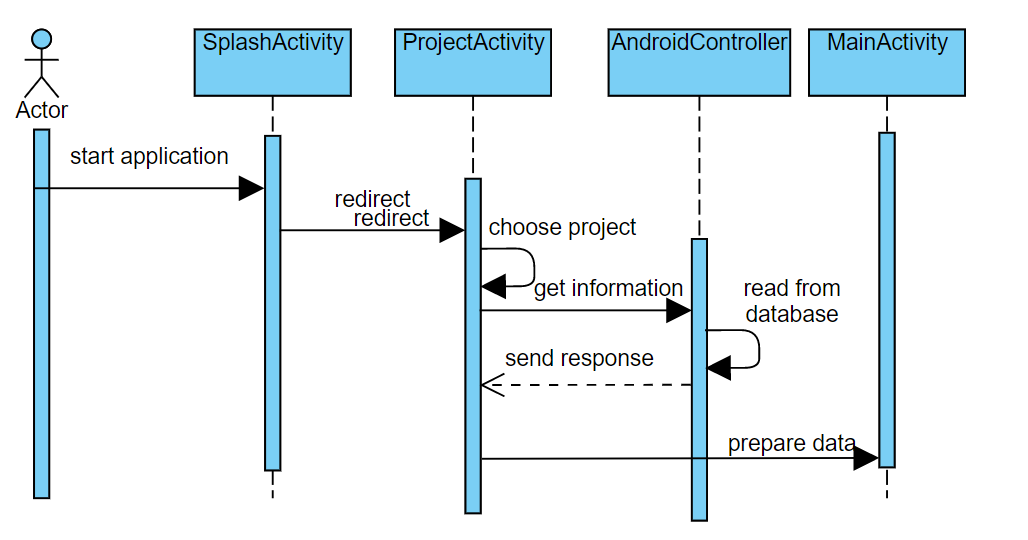
\includegraphics[height=8cm]{images/seqAct.PNG}
  % The short caption should be capitalised
  % The full caption should hold a full sentence. 
 \caption[Sequenzdiagramm für die Interaktion der verschiedenen Activities untereinander und mit der Webapplikation.]{Sequenzdiagramm für die Interaktion der verschiedenen Activities untereinander und mit der Webapplikation (Controller).}
  \label{fig:popup}
\end{figure}


\chapterend % implementation, prototype
%%%%%%%%%%%%%%%%%%%%%%%%%%%%%%%%%%%%%%%%%%%%%%%%%%%%%%%%%%%%%%%%%%%%%%%%%%%%%
\chapter{Evaluation}
\label{Evaluierung}
%%%%%%%%%%%%%%%%%%%%%%%%%%%%%%%%%%%%%%%%%%%%%%%%%%%%%%%%%%%%%%%%%%%%%%%%%%%%%
\chapterstart
\section{Vergleich der neuen Features mit anderen Lösungen}
Dieser Vergleich setzt den Vergleich mit herkömmlichen Lösungen aus dem ersten Teil dieser Arbeit fort (Code Qualität und der Einsatz der Statischen Code Analyse für weitere Auswertungen und Präsentationen der Daten, Punkt 5.1):

\begin{itemize} 
\item Neue Benutzerinnen oder Benutzer können zum Projekt und damit zum Team hinzugefügt werden. Diese können von Administratoren hinzugefügt werden. Andere Lösungen wie integrierte Lösungen in Entwicklungsumgebungen oder Lösungen in der CI-Pipeline unterstützen diese Teamfunktionalität nicht. Hingegen unterstützen Produkte wie Veracode\footnote{https://help.veracode.com/reader/RXjxbTR2MDQdN3gX4l53CQ/RI1a2OsFNYfLuMX2t9BEOg} oder SonarQube\footnote{https://docs.sonarqube.org/latest/instance-administration/security/} dieses Funktionalität.
\item Produkte wie SonarQube unterstützen auch eine genaue Rollenverwaltung für spezielle Funktionen in der Applikation. Diese ist in dieser Arbeit hingegen nicht implementiert.
\item Durch die Github-Anbindung können für einzelne Benutzerinnen oder Benutzer die persönlichen Fehler angezeigt werden. Andere Lösungen unterstützen diese Funktionalität nicht. SonarQube und Veracode unterstützen aber eine Github-Anbindung, mit der beispielsweise die Pull Request und damit der neue Code gezielt untersucht werden können.
\item Mit dem Report-Tool kann nun an das Team oder an andere Personen automatisch ein generierter Report mit den wichtigsten Informationen gesendet werden. Reports können auch von integrierten Tools für Entwicklungsumgebungen erstellt, aber nicht automatisch versendet werden.
\item Mit der Kommentar-Funktion können Kommentare zu den einzelnen Meldungen erfasst und vom ganzen Team eingesehen werden. Diese Funktionalität wird auch von SonarQube, aber nicht von Veracode oder integrierten Lösungen unterstützt.
\item Mit der mobilen Android-Lösung können die wichtigsten Informationen einfach und schnell vom Team gesehen werden. Eine solche Möglichkeit wird von keiner anderen Lösung unterstützt.
\end{itemize}

\section{Evaluierung der Applikationen anhand von Testpersonen}
Die Kriterien, die in Punkt 1.2.2 beschrieben werden, werden von Testpersonen mit den Noten 1-5 bewertet. Ebenso werden die Anmerkungen von den Testpersonen festgehalten. Die Testpersonen arbeiten dazu zusammen mit der Applikation. Für die Testpersonen wird ein eigenes Team erstellt. Im Testablauf wird neuer fehlerhafter Code committed, danach der Fehler angezeigt und ausgebessert. Auch soll der Fehler in der mobilen Applikation angezeigt werden. Zum Fehler werden auch Kommentare erstellt, die von den anderen Teammitgliedern eingesehen werden können.
\subsection{Testpersonen}
Für die Evaluierung wurden aus Testpersonen zwei Teams gebildet.
\subsubsection{Evaluierung durch das erste Team}
Das \textit{Team 1} bestand aus drei Testpersonen. \\
\textbf{Einfachheit} \\
Testperson 1: 1, Code schon in der UI anzeigen, nicht über die Navigation \\
Testperson 2: 3, Standard-Daten schon anzeigen, zum Beispiel Filterung der Meldung des letzten Commits \\
Testperson 3: 2, Längere Erklärungen und Informationen bei den einzelnen Unterseiten und Funktionen \\
\textbf{Übersicht} \\
Testperson 1: 1 \\
Testperson 2: 2 \\
Testperson 3: 2, Unterseiten auch für Charts und Bilder \\
\textbf{Unterstützung} \\
Testperson 1: 1 \\
Testperson 2: 2 \\
Testperson 3: 1, Unterseiten auch für Charts und Bilder \\
\textbf{Individualität} \\
Testperson 1: 1 \\
Testperson 2: 3, Anbindung auch an andere VCS-Tools, Bereitstellung einer API um andere Tools einfach zu unterstützen \\
Testperson 3: 2, Cron-Job Zeiten sollen in der Weboberfläche selber zum Einrichten sein\\
\textbf{Performance} \\
Testperson 1: 1 \\
Testperson 2: 1 \\
Testperson 3: 1 \\
\textbf{Verständlichkeit} \\
Testperson 1: 1 \\
Testperson 2: 2, Information über Shake-Funktion in der Android-Applikation anzeigen \\
Testperson 3: 2, Mehr Erklärungen zu den einzelnen Charts (auch in der Android-Applikation) \\
\textbf{Unterstützung für das Team} \\
Testperson 1: 2, Bereitstellen eines Filters für Meldungen mit Kommentaren \\
Testperson 2: 1, Anbinden eines Kanban-Boards für Verfolgen des Fortschritts der Fehlerausbesserung \\
Testperson 3: 1 \\
\subsubsection{Team 2}
Das \textit{Team 2} bestand aus zwei Testpersonen. \\
\textbf{Einfachheit} \\
Testperson 1: 3, Mehr Information initial anzeigen, zum Beispiel in einem Dashboard  \\
Testperson 2: 3, Andere Implementierung für Fehlerimport, zum Beispiel automatisch durch Repository-Angabe\\
\textbf{Übersicht} \\
Testperson 1: 2, Mehr Informationen auf der initialen  Startseite, zum Beispiel Quicklinks mit Erklärungen für die wichtigsten Funktionen\\
Testperson 2: 1, Erstellen eines User-Dashboards. Dort können die Projekte des Users und Informationen wie häufigste Fehler angezeigt werden.\\
\textbf{Unterstützung} \\
Testperson 1: 2, Implementierung einer automatischen Lösungssuche mittels Schlüsselwörtern.  \\
Testperson 2: 2, Hinzufügen einer Einstufung für die Wichtigkeit der Meldungen\\
\textbf{Individualität} \\
Testperson 1: 2, Cron-Zeiten in der Weboberfläche automatisch anpassen; Hinzufügen einer Möglichkeit zur Erstellung von Labels (Datenbank, Architektur, UI, ...), die Meldungen zugeordnet werden können.\\
Testperson 2: 1 \\
\textbf{Performance} \\
Testperson 1: 2 \\
Testperson 2: 1 \\
\textbf{Verständlichkeit} \\
Testperson 1: 1, Segmente statt den Footer in der Android-Applikation erstellen. Icons für die Navigation neben den Meldungen. \\
Testperson 2: 1, Erstellen einer Dokumentation \\
\textbf{Unterstützung für das Team} \\
Testperson 1: 2, Implementierung der Möglichkeit zum Zuweisen von einzelnen Meldungen zu Benutzerinnen oder Benutzern\\
Testperson 2: 2, Hinzufügen einer besseren Interaktion durch Nachrichten, die an die Teammitglieder geschickt werden können; 
\subsection{Interpretation der Evaluierungen}
\textbf{Einfachheit}: Durchschnittliche Wert: 2,4\\
Viele Testpersonen merkten die fehlende initiale Anzeige an. Mit einer initialen Standardanzeige könnten ohne Abfrage die wichtigsten neuesten Meldungen und Informationen angezeigt werden. Dies gilt sowohl für die Webapplikation, als auch für die mobile Applikation. Eine zusätzliche Dokumentation soll zusätzlich zum Verständnis und zur Einfachheit beitragen.\\
\textbf{Übersicht}: Durchschnittliche Wert: 1,6\\
Mir der Erstellung eines Dashboards und weiteren Unterseiten kann die Übersicht gesteigert werden. Zusätzlich sollen die Charts auch für die einzelnen Benutzerinnen und Benutzer angepasst werden.\\
\textbf{Unterstützung}: Durchschnittliche Wert: 1,6\\
Mit einer automatischen Lösungssuche kann die Unterstützung noch besser erfolgen. Sie könnte mit Schlüsselwerten entwickelt werden. Ebenso sollen die Meldungen nach Wichtigkeit gereiht werden können, um dringende Fehler schneller sehen zu können. \\
\textbf{Individualität}: Durchschnittliche Wert: 1,8\\
Der hohe Wert des Kriteriums der Individualität zeigt die Möglichkeit auf, das Projekt in unterschiedlichen Projekten einsetzen zu können. Mehr Möglichkeiten zur Konfiguration, wie die Einstellung der Cron-Job Zeiten oder die Anbindungen weiterer VCS-Tools könnte die Individualität der Applikation weiter steigern. \\
\textbf{Performance}: Durchschnittliche Wert: 1,2\\
Bei der Performance gab es mit dem Testsetup keine Problem. Nur bei der Webapplikation gab es leichte Verzögerungen wegen der Requests. \\
\textbf{Verständlichkeit}: Durchschnittliche Wert: 1,4\\
Die Funktionen sollen besser erklärt werden, um die Verständlichkeit zu erhöhen. Ebenso sollen weitere UI-Elemente in der Android-Applikation hinzugefügt werden.\\
\textbf{Unterstützung für Teams}: Durchschnittliche Wert: 1,6\\
Der Wert der Unterstützung für Teams zeigt, die Möglichkeit zur Anwendung der Unterstützung für das Team. Aber auch hier können weitere Möglichkeiten zur Interaktion implementiert werden, wie die Zuweisung von Meldungen zu Usern oder die Anbindung eines eigenen Kanban-Boards für die Meldungen. \\
\chapterend
     % evaluation of prototype
%%%%%%%%%%%%%%%%%%%%%%%%%%%%%%%%%%%%%%%%%%%%%%%%%%%%%%%%%%%%%%%%%%%%%%%%%%%%%
\chapter{Conclusion and Outlook}
\label{chap:conclusion}
%%%%%%%%%%%%%%%%%%%%%%%%%%%%%%%%%%%%%%%%%%%%%%%%%%%%%%%%%%%%%%%%%%%%%%%%%%%%%
\chapterstart

neue funktionen in der app (punktesystem) , download der charts in der applikatioin, einloggen android;    generieren der charts unabhängig von der ui 

\chapterend



%%
% Hints by Daniela Holzer 2017
% "instructions for composing degree papers.pdf"
%
% Formal Guidelines
%   Diploma thesis: 17 000 words ± 10% (excluding appendix)
%   Each of the two Bachelor papers: 10 000 words ± 10% (excluding appendix)
%%      % summary, your conclusions/outlook

%\appendix
%%%%%%%%%%%%%%%%%%%%%%%%%%%%%%%%%%%%%%%%%%%%%%%%%%%%%%%%%%%%%%%%%%%%%%%%%%%%%%
\chapter*{Acronyms} % Note the * with \chapter*, which hides it from TOC
\label{chap:acronyms}
%%%%%%%%%%%%%%%%%%%%%%%%%%%%%%%%%%%%%%%%%%%%%%%%%%%%%%%%%%%%%%%%%%%%%%%%%%%%%
% Which one will be the longest ...?
% ABCDE --> \begin{acronym}[ABCDE]
\footnotesize
\begin{acronym}[ABCDE]
  \acro{ABI} {Application Binary Interface}
  \acro{ACL} {Access Control List}
  \acro{GUI} {Graphical User Interface}
  \acro{KISS}{Keep It Small and Simple}
  \acro{MITM}{Man-In-The-Middle}
  \acro{OS}  {Operating System}
  \acro{UART}{Universal Asynchronous Receiver/Transmitter}
  \acro{UID} {Unique Identifier}
\end{acronym}
\normalsize
       % optional

%\TODO{Finally, check the bibliography. Are you sure, that everyone can find the given resources with the information you supplied? Besides author and  year, for books you need the publisher information and the ISBN, for IEEE/ACM research papers add the conference title, location and the DOI.}
\printbibliography

% Adding entry "References" to TOC
% LaTeX-Note: this entry must be added after \printbibliography
%             to get a working link in the TOC!
\addcontentsline{toc}{chapter}{Literatur}

\end{document}


%**********************************************************************
%**********************************************************************
